\chapter{智力题}

\noindent 保加利亚单人纸牌问题:

取出 $ N $ 张牌, 其中 $ N = 1 + 2 + \cdots + k $ 是一个三角形数, 然后把它们随意分成若干堆. 接下来, 从每一堆里各取一张牌, 叠在一起形成一堆新的牌. 不断这样做下去, 如果某个时候桌面上正好有 $ k $ 堆牌, 并且各堆牌数分别为 $ 1,2,3,4,\cdots,k $, 你就获胜了. 要证明不管初始牌堆如何, 有限次操作后一定能达到目标.

\begin{figure*}[htbp]
\centering
\definecolor{rvwvcq}{rgb}{0.08235294117647059,0.396078431372549,0.7529411764705882}
\begin{tabular}{llll} 
\begin{tikzpicture}[line cap=round,line join=round,>=triangle 45,x=1cm,y=1cm,scale=0.6]
\clip(-0.1,-0.1) rectangle (5.1,5.1);
\draw [line width=1pt] (0,5)-- (1,5);
\draw [line width=1pt] (1,5)-- (1,0);
\draw [line width=1pt] (0,0)-- (0,5);
\draw [line width=1pt] (0,4)-- (2,4);
\draw [line width=1pt] (2,4)-- (2,0);
\draw [line width=1pt] (0,3)-- (3,3);
\draw [line width=1pt] (3,3)-- (3,0);
\draw [line width=1pt] (0,2)-- (4,2);
\draw [line width=1pt] (4,2)-- (4,0);
\draw [line width=1pt] (0,1)-- (5,1);
\draw [line width=1pt] (5,1)-- (5,0);
\draw [line width=1pt] (0,0)-- (5,0);
\draw [line width=1pt,dash pattern=on 5pt off 5pt,color=rvwvcq,draw opacity=0.5] (0,1)-- (1,0);
\draw [line width=1pt,dash pattern=on 5pt off 5pt,color=rvwvcq,draw opacity=0.5] (2,0)-- (0,2);
\draw [line width=1pt,dash pattern=on 5pt off 5pt,color=rvwvcq,draw opacity=0.5] (0,3)-- (3,0);
\draw [line width=1pt,dash pattern=on 5pt off 5pt,color=rvwvcq,draw opacity=0.5] (4,0)-- (0,4);
\draw [line width=1pt,dash pattern=on 5pt off 5pt,color=rvwvcq,draw opacity=0.5] (0,5)-- (5,0);
\draw (0.5,0.5) node[anchor=center] {$a$};
\draw (0.5,1.5) node[anchor=center] {$b$};
\draw (0.5,2.5) node[anchor=center] {$c$};
\draw (0.5,3.5) node[anchor=center] {$d$};
\draw (0.5,4.5) node[anchor=center] {$e$};
\draw (1.5,0.5) node[anchor=center] {$f$};
\draw (1.5,1.5) node[anchor=center] {$g$};
\draw (1.5,2.5) node[anchor=center] {$h$};
\draw (2.5,0.5) node[anchor=center] {$i$};
\draw (3.5,0.5) node[anchor=center] {$j$};
\end{tikzpicture}
&
\begin{tikzpicture}[line cap=round,line join=round,>=triangle 45,x=1cm,y=1cm,scale=0.6]
\clip(-0.1,-0.1) rectangle (5.1,5.1);
\draw [line width=1pt] (0,5)-- (1,5);
\draw [line width=1pt] (1,5)-- (1,0);
\draw [line width=1pt] (0,0)-- (0,5);
\draw [line width=1pt] (0,4)-- (2,4);
\draw [line width=1pt] (2,4)-- (2,0);
\draw [line width=1pt] (0,3)-- (3,3);
\draw [line width=1pt] (3,3)-- (3,0);
\draw [line width=1pt] (0,2)-- (4,2);
\draw [line width=1pt] (4,2)-- (4,0);
\draw [line width=1pt] (0,1)-- (5,1);
\draw [line width=1pt] (5,1)-- (5,0);
\draw [line width=1pt] (0,0)-- (5,0);
\draw [line width=1pt,dash pattern=on 5pt off 5pt,color=rvwvcq,draw opacity=0.5] (0,1)-- (1,0);
\draw [line width=1pt,dash pattern=on 5pt off 5pt,color=rvwvcq,draw opacity=0.5] (2,0)-- (0,2);
\draw [line width=1pt,dash pattern=on 5pt off 5pt,color=rvwvcq,draw opacity=0.5] (0,3)-- (3,0);
\draw [line width=1pt,dash pattern=on 5pt off 5pt,color=rvwvcq,draw opacity=0.5] (4,0)-- (0,4);
\draw [line width=1pt,dash pattern=on 5pt off 5pt,color=rvwvcq,draw opacity=0.5] (0,5)-- (5,0);
\draw (0.5,0.5) node[anchor=center] {$a$};
\draw (0.5,1.5) node[anchor=center] {$f$};
\draw (0.5,2.5) node[anchor=center] {$i$};
\draw (0.5,3.5) node[anchor=center] {$j$};
\draw (1.5,0.5) node[anchor=center] {$b$};
\draw (1.5,1.5) node[anchor=center] {$c$};
\draw (1.5,2.5) node[anchor=center] {$d$};
\draw (1.5,3.5) node[anchor=center] {$e$};
\draw (2.5,0.5) node[anchor=center] {$g$};
\draw (2.5,1.5) node[anchor=center] {$h$};
\end{tikzpicture}
&
\begin{tikzpicture}[line cap=round,line join=round,>=triangle 45,x=1cm,y=1cm,scale=0.6]
\clip(-0.1,-0.1) rectangle (5.1,5.1);
\draw [line width=1pt] (0,5)-- (1,5);
\draw [line width=1pt] (1,5)-- (1,0);
\draw [line width=1pt] (0,0)-- (0,5);
\draw [line width=1pt] (0,4)-- (2,4);
\draw [line width=1pt] (2,4)-- (2,0);
\draw [line width=1pt] (0,3)-- (3,3);
\draw [line width=1pt] (3,3)-- (3,0);
\draw [line width=1pt] (0,2)-- (4,2);
\draw [line width=1pt] (4,2)-- (4,0);
\draw [line width=1pt] (0,1)-- (5,1);
\draw [line width=1pt] (5,1)-- (5,0);
\draw [line width=1pt] (0,0)-- (5,0);
\draw [line width=1pt,dash pattern=on 5pt off 5pt,color=rvwvcq,draw opacity=0.5] (0,1)-- (1,0);
\draw [line width=1pt,dash pattern=on 5pt off 5pt,color=rvwvcq,draw opacity=0.5] (2,0)-- (0,2);
\draw [line width=1pt,dash pattern=on 5pt off 5pt,color=rvwvcq,draw opacity=0.5] (0,3)-- (3,0);
\draw [line width=1pt,dash pattern=on 5pt off 5pt,color=rvwvcq,draw opacity=0.5] (4,0)-- (0,4);
\draw [line width=1pt,dash pattern=on 5pt off 5pt,color=rvwvcq,draw opacity=0.5] (0,5)-- (5,0);
\draw (0.5,0.5) node[anchor=center] {$a$};
\draw (0.5,1.5) node[anchor=center] {$b$};
\draw (0.5,2.5) node[anchor=center] {$g$};
\draw (1.5,0.5) node[anchor=center] {$f$};
\draw (1.5,1.5) node[anchor=center] {$i$};
\draw (1.5,2.5) node[anchor=center] {$j$};
\draw (2.5,0.5) node[anchor=center] {$c$};
\draw (2.5,1.5) node[anchor=center] {$d$};
\draw (2.5,2.5) node[anchor=center] {$e$};
\draw (3.5,0.5) node[anchor=center] {$h$};
\end{tikzpicture}
&
\begin{tikzpicture}[line cap=round,line join=round,>=triangle 45,x=1cm,y=1cm,scale=0.6]
\clip(-0.1,-0.1) rectangle (5.1,5.1);
\draw [line width=1pt] (0,5)-- (1,5);
\draw [line width=1pt] (1,5)-- (1,0);
\draw [line width=1pt] (0,0)-- (0,5);
\draw [line width=1pt] (0,4)-- (2,4);
\draw [line width=1pt] (2,4)-- (2,0);
\draw [line width=1pt] (0,3)-- (3,3);
\draw [line width=1pt] (3,3)-- (3,0);
\draw [line width=1pt] (0,2)-- (4,2);
\draw [line width=1pt] (4,2)-- (4,0);
\draw [line width=1pt] (0,1)-- (5,1);
\draw [line width=1pt] (5,1)-- (5,0);
\draw [line width=1pt] (0,0)-- (5,0);
\draw [line width=1pt,dash pattern=on 5pt off 5pt,color=rvwvcq,draw opacity=0.5] (0,1)-- (1,0);
\draw [line width=1pt,dash pattern=on 5pt off 5pt,color=rvwvcq,draw opacity=0.5] (2,0)-- (0,2);
\draw [line width=1pt,dash pattern=on 5pt off 5pt,color=rvwvcq,draw opacity=0.5] (0,3)-- (3,0);
\draw [line width=1pt,dash pattern=on 5pt off 5pt,color=rvwvcq,draw opacity=0.5] (4,0)-- (0,4);
\draw [line width=1pt,dash pattern=on 5pt off 5pt,color=rvwvcq,draw opacity=0.5] (0,5)-- (5,0);
\draw (0.5,0.5) node[anchor=center] {$a$};
\draw (0.5,1.5) node[anchor=center] {$f$};
\draw (0.5,2.5) node[anchor=center] {$c$};
\draw (0.5,3.5) node[anchor=center] {$h$};
\draw (1.5,0.5) node[anchor=center] {$b$};
\draw (1.5,1.5) node[anchor=center] {$g$};
\draw (2.5,0.5) node[anchor=center] {$i$};
\draw (2.5,1.5) node[anchor=center] {$j$};
\draw (3.5,0.5) node[anchor=center] {$d$};
\draw (3.5,1.5) node[anchor=center] {$e$};
\end{tikzpicture}
\\
\begin{tikzpicture}[line cap=round,line join=round,>=triangle 45,x=1cm,y=1cm,scale=0.6]
\clip(-0.1,-0.1) rectangle (5.1,5.1);
\draw [line width=1pt] (0,5)-- (1,5);
\draw [line width=1pt] (1,5)-- (1,0);
\draw [line width=1pt] (0,0)-- (0,5);
\draw [line width=1pt] (0,4)-- (2,4);
\draw [line width=1pt] (2,4)-- (2,0);
\draw [line width=1pt] (0,3)-- (3,3);
\draw [line width=1pt] (3,3)-- (3,0);
\draw [line width=1pt] (0,2)-- (4,2);
\draw [line width=1pt] (4,2)-- (4,0);
\draw [line width=1pt] (0,1)-- (5,1);
\draw [line width=1pt] (5,1)-- (5,0);
\draw [line width=1pt] (0,0)-- (5,0);
\draw [line width=1pt,dash pattern=on 5pt off 5pt,color=rvwvcq,draw opacity=0.5] (0,1)-- (1,0);
\draw [line width=1pt,dash pattern=on 5pt off 5pt,color=rvwvcq,draw opacity=0.5] (2,0)-- (0,2);
\draw [line width=1pt,dash pattern=on 5pt off 5pt,color=rvwvcq,draw opacity=0.5] (0,3)-- (3,0);
\draw [line width=1pt,dash pattern=on 5pt off 5pt,color=rvwvcq,draw opacity=0.5] (4,0)-- (0,4);
\draw [line width=1pt,dash pattern=on 5pt off 5pt,color=rvwvcq,draw opacity=0.5] (0,5)-- (5,0);
\draw (0.5,0.5) node[anchor=center] {$a$};
\draw (0.5,1.5) node[anchor=center] {$b$};
\draw (0.5,2.5) node[anchor=center] {$i$};
\draw (0.5,3.5) node[anchor=center] {$d$};
\draw (1.5,0.5) node[anchor=center] {$f$};
\draw (1.5,1.5) node[anchor=center] {$c$};
\draw (1.5,2.5) node[anchor=center] {$h$};
\draw (2.5,0.5) node[anchor=center] {$g$};
\draw (3.5,0.5) node[anchor=center] {$j$};
\draw (4.5,0.5) node[anchor=center] {$e$};
\end{tikzpicture}
&
\begin{tikzpicture}[line cap=round,line join=round,>=triangle 45,x=1cm,y=1cm,scale=0.6]
\clip(-0.1,-0.1) rectangle (5.1,5.1);
\draw [line width=1pt] (0,5)-- (1,5);
\draw [line width=1pt] (1,5)-- (1,0);
\draw [line width=1pt] (0,0)-- (0,5);
\draw [line width=1pt] (0,4)-- (2,4);
\draw [line width=1pt] (2,4)-- (2,0);
\draw [line width=1pt] (0,3)-- (3,3);
\draw [line width=1pt] (3,3)-- (3,0);
\draw [line width=1pt] (0,2)-- (4,2);
\draw [line width=1pt] (4,2)-- (4,0);
\draw [line width=1pt] (0,1)-- (5,1);
\draw [line width=1pt] (5,1)-- (5,0);
\draw [line width=1pt] (0,0)-- (5,0);
\draw [line width=1pt,dash pattern=on 5pt off 5pt,color=rvwvcq,draw opacity=0.5] (0,1)-- (1,0);
\draw [line width=1pt,dash pattern=on 5pt off 5pt,color=rvwvcq,draw opacity=0.5] (2,0)-- (0,2);
\draw [line width=1pt,dash pattern=on 5pt off 5pt,color=rvwvcq,draw opacity=0.5] (0,3)-- (3,0);
\draw [line width=1pt,dash pattern=on 5pt off 5pt,color=rvwvcq,draw opacity=0.5] (4,0)-- (0,4);
\draw [line width=1pt,dash pattern=on 5pt off 5pt,color=rvwvcq,draw opacity=0.5] (0,5)-- (5,0);
\draw (0.5,0.5) node[anchor=center] {$a$};
\draw (0.5,1.5) node[anchor=center] {$f$};
\draw (0.5,2.5) node[anchor=center] {$g$};
\draw (0.5,3.5) node[anchor=center] {$j$};
\draw (0.5,4.5) node[anchor=center] {$e$};
\draw (1.5,0.5) node[anchor=center] {$b$};
\draw (1.5,1.5) node[anchor=center] {$i$};
\draw (1.5,2.5) node[anchor=center] {$d$};
\draw (2.5,0.5) node[anchor=center] {$c$};
\draw (2.5,1.5) node[anchor=center] {$h$};
\end{tikzpicture}
&
\begin{tikzpicture}[line cap=round,line join=round,>=triangle 45,x=1cm,y=1cm,scale=0.6]
\clip(-0.1,-0.1) rectangle (5.1,5.1);
\draw [line width=1pt] (0,5)-- (1,5);
\draw [line width=1pt] (1,5)-- (1,0);
\draw [line width=1pt] (0,0)-- (0,5);
\draw [line width=1pt] (0,4)-- (2,4);
\draw [line width=1pt] (2,4)-- (2,0);
\draw [line width=1pt] (0,3)-- (3,3);
\draw [line width=1pt] (3,3)-- (3,0);
\draw [line width=1pt] (0,2)-- (4,2);
\draw [line width=1pt] (4,2)-- (4,0);
\draw [line width=1pt] (0,1)-- (5,1);
\draw [line width=1pt] (5,1)-- (5,0);
\draw [line width=1pt] (0,0)-- (5,0);
\draw [line width=1pt,dash pattern=on 5pt off 5pt,color=rvwvcq,draw opacity=0.5] (0,1)-- (1,0);
\draw [line width=1pt,dash pattern=on 5pt off 5pt,color=rvwvcq,draw opacity=0.5] (2,0)-- (0,2);
\draw [line width=1pt,dash pattern=on 5pt off 5pt,color=rvwvcq,draw opacity=0.5] (0,3)-- (3,0);
\draw [line width=1pt,dash pattern=on 5pt off 5pt,color=rvwvcq,draw opacity=0.5] (4,0)-- (0,4);
\draw [line width=1pt,dash pattern=on 5pt off 5pt,color=rvwvcq,draw opacity=0.5] (0,5)-- (5,0);
\draw (0.5,0.5) node[anchor=center] {$a$};
\draw (0.5,1.5) node[anchor=center] {$b$};
\draw (0.5,2.5) node[anchor=center] {$c$};
\draw (1.5,0.5) node[anchor=center] {$f$};
\draw (1.5,1.5) node[anchor=center] {$g$};
\draw (1.5,2.5) node[anchor=center] {$j$};
\draw (1.5,3.5) node[anchor=center] {$e$};
\draw (2.5,0.5) node[anchor=center] {$i$};
\draw (2.5,1.5) node[anchor=center] {$d$};
\draw (3.5,0.5) node[anchor=center] {$h$};
\end{tikzpicture}
&
\begin{tikzpicture}[line cap=round,line join=round,>=triangle 45,x=1cm,y=1cm,scale=0.6]
\clip(-0.1,-0.1) rectangle (5.1,5.1);
\draw [line width=1pt] (0,5)-- (1,5);
\draw [line width=1pt] (1,5)-- (1,0);
\draw [line width=1pt] (0,0)-- (0,5);
\draw [line width=1pt] (0,4)-- (2,4);
\draw [line width=1pt] (2,4)-- (2,0);
\draw [line width=1pt] (0,3)-- (3,3);
\draw [line width=1pt] (3,3)-- (3,0);
\draw [line width=1pt] (0,2)-- (4,2);
\draw [line width=1pt] (4,2)-- (4,0);
\draw [line width=1pt] (0,1)-- (5,1);
\draw [line width=1pt] (5,1)-- (5,0);
\draw [line width=1pt] (0,0)-- (5,0);
\draw [line width=1pt,dash pattern=on 5pt off 5pt,color=rvwvcq,draw opacity=0.5] (0,1)-- (1,0);
\draw [line width=1pt,dash pattern=on 5pt off 5pt,color=rvwvcq,draw opacity=0.5] (2,0)-- (0,2);
\draw [line width=1pt,dash pattern=on 5pt off 5pt,color=rvwvcq,draw opacity=0.5] (0,3)-- (3,0);
\draw [line width=1pt,dash pattern=on 5pt off 5pt,color=rvwvcq,draw opacity=0.5] (4,0)-- (0,4);
\draw [line width=1pt,dash pattern=on 5pt off 5pt,color=rvwvcq,draw opacity=0.5] (0,5)-- (5,0);
\draw (0.5,0.5) node[anchor=center] {$a$};
\draw (0.5,1.5) node[anchor=center] {$b$};
\draw (0.5,2.5) node[anchor=center] {$c$};
\draw (0.5,3.5) node[anchor=center] {$e$};
\draw (1.5,0.5) node[anchor=center] {$f$};
\draw (1.5,1.5) node[anchor=center] {$g$};
\draw (1.5,2.5) node[anchor=center] {$j$};
\draw (2.5,0.5) node[anchor=center] {$i$};
\draw (2.5,1.5) node[anchor=center] {$d$};
\draw (3.5,0.5) node[anchor=center] {$h$};
\end{tikzpicture}
\end{tabular}
\end{figure*}

上图示意了一个操作序列. 先把所有的牌堆按数量从多到少排列, 最多的在最左边. 每次从每一堆取最下面一张牌, 形成的新牌堆放在最左边, 再调整牌堆的次序使得它们仍然按从多到少的顺序排列. 

考虑上图的几条对角线, 每条对角线上的牌视为一组, 左下角的 $ a $ 为第 1 组, $ b, f $ 为第 2 组, 等等. 观察所有牌的组号之和在操作过程中会怎样变化.

组成新牌堆时, 最下面一行牌挪到的各自对角线的最左侧. 其他牌沿着对角线往右下移动一格, 相当于每条对角线上的牌循环移动了一格. 这样的操作里每条对角线上的牌还是原来的那些, 所以所有牌的组号之和不变.

需要调整牌堆顺序时, 一定是右边一堆牌数量多于左边的一堆, 这时将右边多出的部分挪到左边, 这部分牌都被移到编号更小的组里, 所以组号之和减小.

因为各堆牌数量之组合的可能状态是有限的, 经过足够多次的操作后一定能遇到之前的某个状态, 这样状态就会产生循环. 一次循环后又回到同一状态, 而前面已经说明组号之和只能不变或减小, 不可能增大, 如果出现调整牌堆顺序, 组号之和会减小, 于是在一个循环里, 不会出现调整牌堆顺序的操作.

也就是说, 一个循环中, 每个操作都是循环移动各对角线上的牌. 

如果一条对角线 $ i $ 上有一个牌 $ x $, 同时它的前一条对角线 $ i - 1 $ 上有一个空位 $ y $. 两条对角线上牌的循环移位周期相差 1, 所以 $ x $ 总能和 $ y $ 到达同一高度, $ x $ 在 $ y $ 的正右方, 这将引起一次牌堆顺序调整. 所以这种情况不会发生在一个状态循环里.

所以在状态循环里, 每条对角线上都是满的, 除了最后一个对角线外. 但是牌的总数是三角形数, 这样最后一个对角线也是满的. 所以循环只可能是 $ (k,k-1,\cdots,2,1) $. 而无论什么初始状态都会进入循环, 所以这个游戏总能在有限次操作后达到目标状态.


\newpage
%------------------------------------------------------------------------------%
\noindent 环球城市数学竞赛~ 1980 春季~ 初中组/高中组

在一个 $ N \times N $ 的矩阵中, 这 $ N $ 行是两两不相等的. 只要有一列不相等就称这两行不相等. 
求证: 存在某一列, 去掉这一列后剩下的 $ N $ 行仍然两两不相等.

~

证明: 用归纳法, 先证明矩阵的前 $ m $ 行中, 最多只要选出 $ m - 1 $ 列, 就能满足这 $ m $ 行两两不等.

对于 $ m = 2 $ 时, 因为矩阵的行两两不等, 所以存在一列使得前两行在这一列上的数不相等. 

对于 $ m = k $ 时, 存在 $ k - 1 $ 个列, 使得由前 $ k $ 行和这 $ k - 1 $ 个列组成的子矩阵的行向量两两不等. 考虑第 $ k + 1 $ 行, 分两种情况:

(i) 取前 $ k + 1 $ 行和 $ k - 1 $ 列组成的子矩阵就已经两两行不等了, 归纳假设成立;

(ii) 子矩阵中新加入的第 $ k+1 $ 行和前面的某一行 $ i $ 相等, 但不可能与前面的两行或更多行相等. 这是因为子矩阵前 $ k $ 行是两两不等的. 又由题设, 在原来的大矩阵中, 第 $ k + 1 $ 行和第 $ i $ 行存在一列不相等, 把这一列加进子矩阵中, 则新的子矩阵也满足行向量两两不等.

这个过程持续到 $ m = N $ 的时候, 就证明了题设条件下, 只要 $ N - 1 $ 列就满足行向量两两不等.

\newpage
%------------------------------------------------------------------------------%
证明: 对于任意正整数 $k$, 都存在一个正整数 $n_k$, 使得集合 $S = \{1^2,2^2,\cdots,n_k^2\}$ 中每个元素乘以 1 或 -1 并求和, 其和等于 $k$.

~

解: 对于 $k=1,2,3,4$, 可以分别构造求和式如下:
\begin{align*}
1 &= 1^2 \\
2 &= -1^2 - 2^2 - 3^2 + 4^2\\
3 &= -1^2 + 2^2\\
4 &= -1^2 - 2^2 + 3^2
\end{align*}

下面用归纳法, 注意到
\[(n+1)^2 - (n+2)^2 - (n+3)^2 + (n+4)^2 = 4 .\]
如果对于 $k$, 可以表示成 $\{1^2,\cdots,n_k^2\}$ 乘以 1 或 -1 之和, 则对于 $k+4$, 则可以表示为 $\{1^2,\cdots,(n_k+4)^2\}$ 乘以 1 或 -1 之和. 例如 
\begin{align*}
5 &= 1 + 4 = 1^2 + 2^2 - 3^3 - 4^2 + 5^2 \\ 
6 &= 2 + 4 = -1^2 - 2^2 - 3^2 + 4^2 + 5^2 - 6^2 - 7^2 + 8^2\\
7 &= 3 + 4 = -1^2 + 2^2 + 3^2 - 4^2 - 5^2 + 6^2\\
8 &= 4 + 4 = -1^2 - 2^2 + 3^2 + 4^2 - 5^2 - 6^2 + 7^2
\end{align*}
等等.

\newpage
%------------------------------------------------------------------------------%

\noindent 环球城市数学竞赛~ 1981 春季~ 初中组/高中组

$ A, B $ 两人下棋, 棋盘是无限大的平面, $ A $ 控制 $ N $ 个羊, $ B $ 控制一个狼, 每一步 $ A $ 只能选其中一个羊移动, $B$ 控制狼, $A,B$ 轮流移动, 羊和狼每一步只能移动不超过一米, 但可以沿任意方向, 不必走整点. $ A $ 可以决定开局时狼和羊的位置, 问是否存在一个开局状态, 使得狼抓不到任何一只羊?

~

解: 将第 $ k $ 个羊放在水平线 $ y = kN $ 上, 这里 $ N $ 是一个比较大的数, 比如 $ N = 10 $. 同时将狼摆在离所有羊距离都足够远的地方. 每个羊只在自己所在的水平线上移动. 任意时刻, 狼只要到某条水平线的距离小于 2 米, 就说狼会对这条线上的羊造成威胁, 对应的羊只要朝远离狼的方向移动, 这样狼不会追上这个羊. 而狼最多同时对一只羊造成威胁, 所以羊总是能逃过.

\newpage
%------------------------------------------------------------------------------%
\noindent 环球城市数学竞赛~ 1981 春季~ 高中组

\begin{figure*}[htbp]
\centering
\definecolor{rvwvcq}{rgb}{0.08235294117647059,0.396078431372549,0.7529411764705882}
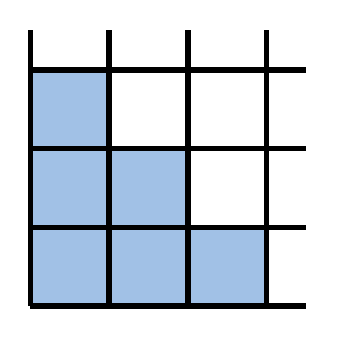
\begin{tikzpicture}[]
\fill[fill=rvwvcq,opacity=0.4] (0,0) -- (0,3) -- (1,3) -- (1,2) -- (2,2) -- (2,1) -- (3,1) -- (3,0) -- cycle;
\draw [line width=2pt,color=black] (-0,-0) grid (3.5,3.5);
\end{tikzpicture}
\end{figure*}

无限大的方格纸上有一些棋子, 每个格子最多有一个棋子, 可以按下面的规则操作: 如果一个棋子的上邻和右邻的格子内都没有棋子, 可以去掉这个棋子, 并在上邻和右邻各放一个棋子. 纸上有 6 个特殊标记的格子, 下面的给出两种开局情况, 问是否能通过有限次操作让这 6 个被标记的方格内都没有棋子:

(a) 整个纸上只有这 6 个被标记的格子中有棋子;

(b) 整个纸上只有左下角被标记的那一个格子内有棋子.

~

解: 给每个格子一个数值, 其中左下角被标记的格子值是 1, 其他格子的值是它左边或下边数值的一半. 
\begin{figure*}[htbp]
\centering
\definecolor{rvwvcq}{rgb}{0.08235294117647059,0.396078431372549,0.7529411764705882}
\begin{tikzpicture}[evaluate={
		int \i, \j;
		for \i in {0,...,4}{
			for \j in {0,...,4}{
				\a{\i,\j} = int((2^(\i+\j)));
			};
		};
	}]
\fill[fill=rvwvcq,opacity=0.4] (0,0) -- (0,3) -- (1,3) -- (1,2) -- (2,2) -- (2,1) -- (3,1) -- (3,0) -- cycle;
\fill[fill=red!30] (0,3) -- (0,5.5) -- (1,5.5) -- (1,3) -- cycle;
\fill[fill=orange!30] (3,0) -- (5.5,0) -- (5.5,1) -- (3,1) -- cycle;
\draw [line width=2pt,color=black] (-0,-0) grid (5.5,5.5);
\foreach \x in {0,...,4}
	\foreach \y in {0,...,4}
		\node at (\x+0.5,\y+0.5) {$\frac{1}{\a{\x,\y}}$};
\end{tikzpicture}
\end{figure*}

当去掉一个棋子时, 会在右边和上边相邻的位置加入一个棋子, 操作前后棋子的数值之和不变. 所有格子的数值之和为
\begin{align*} 
S &= \left(1+\frac{1}{2} + \frac{1}{4} + \cdots \right) + \left(\frac{1}{2} + \frac{1}{4} + \frac{1}{8} + \cdots \right) + \cdots \\
	&= \left( 1+\frac{1}{2} + \frac{1}{4} + \cdots \right) \left( 1+\frac{1}{2} + \frac{1}{4} + \cdots \right) \\
%	&= 2\cdot 2 \\
	&= 4.
\end{align*}

被标记部分的数值之和为 $ 11/4 $, 其余部分数值为 $ 5/4 $, 因为每个格子上最多只能有一个棋子, 所以 (a) 是不可能达到的.

对于 (b) 问题, 初始只有左下角有一个棋子, 不管怎么变, 最左一列和最下一行有且只有一个棋子. 腾空被标记区域后, 这两部分的数值之和最大是 $ 1/4 $, 而剩下白色区域的数值之和是 $ 3/4 $, 如果要达到初始时的数值, 必须白色区域所有格子上都有棋子, 这在有限次操作内是不可能实现的.


\newpage
%------------------------------------------------------------------------------%
\noindent 环球城市数学竞赛~ 1982 春季~ 初中组

设 $\{a_k\}$ 是两两不同, 且每项均大于 1 的无穷整数列. 求证: 在 $\{a_k\}$ 中可以找到无穷多项, 使得 $a_k > k$.

~

思路: 考虑 $a_1$ 的值, 例如假设 $a_1 = 5$, 再看 $a_1, a_2, a_3, a_4, a_5$ 这几个数, 由鸽笼原理, 它们不可能都小于 $5$, 总要有一个数大于 $5$, 找到其中最大的数, 例如是 $a_3=7$, 然后再看 $a_1, \cdots, a_7$, 它们不可能都小于 $7$, 至少有一个会大于 $7$, 再找这 7 个数中的最大值, 例如是 $a_7 = 10$, 这样可以一直构造下去.

~

证明: 可以用归纳构造一个无穷严格递增的正整数序列 $k_1, k_2, \cdots$, 使得对于任意正整数 $n$, 有 $a_{k_n} > k_n$, 且若正整数 $i < k_n$, 则 $a_i < a_{k_n}$.

事实上, $n=1$时, 因为 $a_1 > 1$, 只要取 $k_1 = 1$ 即可. 假设 $k_n$ 已经选好, 因为 $2, 3, \cdots, a_{k_n}$ 是 $a_{k_n} - 1$ 个数, 而 $a_1, a_2, \cdots, a_{a_{k_n}}$ 有 $a_{k_n}$ 个不同的数, 所以它们中至少有一个数大于 $a_{k_n}$. 取 $a_{k_{n+1}} = \max\{a_1, a_2, \cdots, a_{a_{k_n}}\}$, 则 $a_{k_{n+1}} > a_{k_n}$. 而下标 $k_{n+1}$ 是满足 $1 \le k_{n+1} \le a_{k_n}$ 的, 所以有 $a_{k_{n+1}} > a_{k_n} \ge k_{n+1}$. 又因为 $a_{k_{n+1}}$ 是 $a_1, a_2, \cdots, a_{a_{k_n}}$ 中的最大值, 所以当 $i < k_{n+1}$ 时, $a_i < a_{k_{n+1}}$. 

另一方面, 由归纳假设, 当$1\le i \le k_n$ 时,  $a_i \le a_{k_n}$, 但是 $a_{k_{n+1}} > a_{k_n}$, 所以必然有 $k_{n+1} > k_n$, 这就说明了 $k_n$ 是严格单调递增的. 从而存在无穷多个 $k_n$ 满足 $a_{k_n} > k_n$.

\newpage
%------------------------------------------------------------------------------%
\noindent 第 19 届 IMO (1977, 南斯拉夫) 第二题

股东们开会时, 布告栏上展示着上次会议以来的月报表, 或盈或亏, 历历在目. 财务主管说: ``请各位注意, 在任何一个持续八个月的周期内, 我们总是能赚钱的.''

``也许如此吧,'' 有位股东抱怨地说: ``但是我却看到, 在任何一个连续五个月的周期内, 我们总是亏损的!''

问: 上次会议至今, 最多已经过去了几个月份?

~

解: 假设上次会议至今过去了 $n$ 个月, 期间每月收益按时间顺序记为 $a_1, a_2, \cdots, a_n$. 下面证明$n \le 11$.

假设$n\ge 12$, 取前 12 个元素, 排成下面的矩阵:
\[
\begin{bmatrix}
a_1 & a_2 & \cdots & a_8 \\
a_2 & a_3 & \cdots & a_9 \\
\vdots & \vdots & \ddots & \vdots \\
a_5 & a_6 & \cdots & a_{12}
\end{bmatrix}
\]
根据条件, 每行之和都是正数, 于是矩阵所有元素之和为正; 而每列之和都是负数, 则所有元素之和为负, 矛盾了.

另一方面, 可以构造如下的数列在 $n = 11$ 时满足题设条件: 
\[ 5, -8, 5, 5, -8, 5, -8, 5, 5, -8, 5 .\]
所以上次会议最早是11个月前.

\newpage
%------------------------------------------------------------------------------%
\noindent 关于国际象棋棋盘的智力题

~

\noindent 问题:

有一个 $ 8\times 8$ 的网格, 按从左到右从上到下的顺序依次编号 $0, 1, \cdots, 63 $, 再给每个格子涂上黑色或白色, 使得每行每列恰有 $ 4 $ 个白色和 $ 4 $ 个黑色格子. 求证: 白色格子的编号之和等于黑色格子编号之和.

~

\noindent 证明:

只要按八进制写出编号, 第一行格子编号是 $00, 01, \cdots, 07 $, 第二行是 $ 10, 11, \cdots, 17 $ 等等.
因为每行每列恰有 $ 4 $ 个白色格子, 取出所有白色编号, 恰有 $ 4 $ 个低位是 $ 0 $, 恰有 $ 4 $ 个低位是 $ 1 $, 等等, 并且恰有 $ 4 $ 个高位是 $ 0 $, 恰有 $ 4 $ 个高位是 $ 1 $, 等等. 黑色编号也如此, 所以二者的和相等. 

~

\noindent 问题: 

用 $ 32 $ 个 $ 1\times 2 $ 的多米诺骨牌覆盖 $ 8 \times 8 $ 的棋盘, 证明: 无论怎样覆盖, 使用的横的和竖的骨牌数量一定都是偶数个.

~

\noindent 证明:

不失一般性, 逐行考虑每行竖的骨牌个数. 因为每个横的牌能覆盖两个格子, 所以第一行竖的骨牌个数一定是偶数个. 将第一行的这些竖的骨牌拿掉, 这可能会造成第二行有一些 (偶数个) 空隙, 所以第二行剩余的竖的骨牌也是偶数个. 再拿掉第二行剩余的竖的骨牌, 考虑第三行剩余的竖的骨牌, 等等. 这样每一行都拿掉了偶数个竖的骨牌, 到第 $ 8 $ 行时全部拿掉 (其实第 $ 7 $ 行拿掉后就已经没有了). 所以竖的骨牌个数是偶数个. 横的骨牌也是同理.

~

\noindent 问题:

$8\times 8$的标准国际象棋棋盘上任意挖掉一个黑格和一个白格, 证明: 剩下的部分仍然可以用 $ 31 $ 个 $ 1\times 2 $ 的多米诺骨牌完全覆盖.

~

\noindent 证明: 

可以画一条环路经过原棋盘的所有格子, 而不重复, 例如下图就是一种方案.
\begin{figure*}[htbp]
\centering
\begin{tikzpicture}[scale=0.5]
\draw[shift={+(1,1)}] (0,0) -- (0,8) -- (8,8) -- (8,0) -- cycle;
\foreach \x in {2,4,6,8}
	\foreach \y in {2,4,6,8}
		\draw[fill=gray!50] (\x,\y) rectangle ++(1,1);
\foreach \x in {1,3,5,7}
	\foreach \y in {1,3,5,7}
		\draw[fill=gray!50] (\x,\y) rectangle ++(1,1);
\draw [line width=1pt,dashed,shift={+(1,1)}] (0.5,0.5) -- (0.5,7.5) -- (7.5,7.5) -- (7.5,0.5) -- (6.5,0.5) -- (6.5,6.5) -- (5.5,6.5) -- (5.5,0.5) -- (4.5,0.5) -- (4.5,6.5) -- (3.5,6.5) -- (3.5,0.5) -- (2.5,0.5) -- (2.5,6.5) -- (1.5,6.5) -- (1.5,0.5) -- cycle;
\draw[pattern=crosshatch, pattern color=black] (2,5) rectangle ++(1,1);
\draw[pattern=crosshatch, pattern color=black] (5,3) rectangle ++(1,1);
\end{tikzpicture}
\end{figure*}

环路上总是黑白格子交替出现, 任意删掉一黑一白两个格子, 环路被分成两段, 每段路径仍然是一黑一白交替出现, 因此只要用骨牌分别沿着每段路径铺垫, 就可以覆盖剩余的棋盘.


\newpage
%------------------------------------------------------------------------------%
\noindent 来自"Heard on the street"

\noindent 问题: You are given a set of scales and 12 marbles. The scales are of the old balance variety. That is, a small dish hangs from each end of a rod that is balanced in the middle. The device enables you to conclude either that the contents of the dishes weigh the same or that the dish that falls lower has heavier contents than the other.

The 12 marbles appear to be identical. In fact, 11 of them are identical, and one is of a different weight. Your task is to identify the unusual marble and discard it. You are allowed to use the scales three times if you wish, but no more.

Note that the unusual marble may be heavier than the others, or it may be lighter. You are asked to both identify it and determine whether it is heavy or light.

大意: 有 12 个外观一样的石头, 其中 11 个重量是一样的, 剩下的那个可能偏轻或者偏重. 给一个天平, 要用最多 3 次称量找出异常的石头, 以及判断它是偏轻还是偏重. 

~ 

\noindent 解:

把石头编号为 1-12. 用 $ n^+ $ 和 $ n^- $ 表示第 $ n $ 号石头偏重和偏轻的情况, 这样共有 $ 12\times 2 = 24 $ 种可能的异常情况. 我们希望把这些异常情况分成相等的几份, 每次称量筛选出一份, 这样即使在最坏情况下后续的候选情况不至于太多. 

先举一个例子. 显然需要在天平两边放相同数量的石头才有意义. 如果第一次称天平左右两边放 1 号和 2 号. 结果可能有 3 种, 每一种对应的异常情况如下:
\begin{figure*}[htbp]
\centering
\setlength\extrarowheight{2pt}
\begin{tabular}{l|l|l}
\hline
Case 1 & 偏左  & $1^+, 2^-$ \\ \hline
Case 2 & 偏右  & $1^-, 2^+$ \\ \hline
Case 3 & 平衡  & $3^+, 3^-, 4^+, 4^-, 5^+, 5^-, 6^+, 6^-, \cdots, 12^+, 12^- $ \\ \hline
\end{tabular}
\end{figure*}

如果恰好天平平衡了, 需要用 2 次称量分辨 20 种异常情况, 是做不到的. 此外, 经过上表可以观察到, 如果天平偏向某一侧, 则说明这一侧的某个石头可能偏重, 或者对侧的某个石头偏轻. 如果天平平衡说明异常的石头不在天平上. 

我们往两边放更多的石头, 各放 4 个的时候异常情况可以被均分. 例如, 1-4在左边, 5-8在右边, 得到下表:
\begin{figure*}[htbp]
\centering
\setlength\extrarowheight{2pt}
\begin{tabular}{l|l|l}
\hline
Case 1 & 偏左  & $1^+, 2^+, 3^+, 4^+, 5^-, 6^-, 7^-, 8^- $ \\ \hline
Case 2 & 偏右  & $1^-, 2^-, 3^-, 4^-, 5^+, 6^+, 7^+, 8^+ $ \\ \hline
Case 3 & 平衡  & $9^+, 9^-, 10^+, 10^-, 11^+, 11^-, 12^+, 12^- $ \\ \hline
\end{tabular}
\end{figure*}

Case 1 和 Case 2 筛选出来的情况是对称的, 我们选其中偏左的这个结果 (Case 1) 来分析第二次称量的策略. 经过一些尝试, 可以左边放 $\{1,5,9\}$, 右边放 $\{2,3,6\}$. 注意此时如果天平偏左, 说明有 $ \{ 1^+, 5^+, 9^+, 2^-, 3^-, 6^- \}$ 这些可能, 再结合第一次称量的结论, 就只剩下 $ \{1^+, 6^- \} $. 类似的推出偏右和平衡的情况. 最后, 有下表的分析:
\begin{figure*}[htbp]
\centering
\setlength\extrarowheight{2pt}
\begin{tabular}{l|l|l}
\hline
Case 1.1 & 偏左  & $1^+, 6^-$ \\ \hline
Case 1.2 & 偏右  & $2^+, 3^+, 5^- $ \\ \hline
Case 1.3 & 平衡  & $4^+, 7^-, 8^- $ \\ \hline
\end{tabular}
\end{figure*}

对于 Case 1.1, 只要再比较 1 号和 2 号; 平衡对应 $ 6^- $; 偏向 1 号对应 $ 1^+ $, 不会出现偏向 2 号的情况. 

对于 Case 1.2, 比较 2 号和 3 号, 偏向哪个说明哪个是异常, 且偏重; 平衡说明是 $ 5^- $. 

对于 Case 1.3, 比较 7 号和 8 号, 偏向哪个说明另一边是异常, 且更轻; 平衡说明是 $ 4^+ $.

Case 2 和 Case 1是类似的. 

再看 Case 3, 经过一些尝试, 可以左边放 $ \{ 1,9 \} $, 右边放 $ \{ 10, 11 \} $, 得到下表:
\begin{figure*}[htbp]
\centering
\setlength\extrarowheight{2pt}
\begin{tabular}{l|l|l}
\hline
Case 3.1 & 偏左  & $9^+, 10^-, 11^-$ \\ \hline
Case 3.2 & 偏右  & $9^-, 10^+, 11^+ $ \\ \hline
Case 3.3 & 平衡  & $12^+, 12^- $ \\ \hline
\end{tabular}
\end{figure*}

Case 3.1 和 Case 1.3 类似, 而 Case 3.2 和 Case 1.2 类似. 

对于 Case 3.3, 只要比较 1 号和 12 号, 就可知道 12 号是偏轻还是偏重, 同样这里不存在平衡的情况.

~

Heard on the Street 后面之后又提出了一个更复杂的拓展问题: 石头数量变成 90 个, 其中仍然有一个质量与其他的不同, 问至少需要称多少次能在最坏情况下找出, 以及具体方法.

如果仍然向上面那样, 后续的策略要依赖于前面的称量结果进行调整, 就需要逐个情况分析验证, 工作量巨大. 这里借鉴纠错码的思路给出一个通用的解法, 每一步称量策略不依赖于前面的结果.

回到 12 个石头的问题. 我们将称量这一操作用数学的语言描述. 设编号 $ i $ 的石头质量为 $ m_i $, 取值为 $ \{-1,0,1\} $, 分别对应偏轻, 正常, 偏重的情况. 天平的倾斜状态同样可以定义为 $ \{-1, 0, 1\} $, 对应偏左,平衡,偏右的情况, 于是, 每个左盘的石头贡献了负的力矩, 右盘的石头贡献正的力矩. 当然, 对于质量是 $-1$ 的石头则是反过来. 将每个石头放在左盘还是右盘用 $ w_i $ 表示, 同样 $w_i$ 的取值范围是 $ \{-1, 0, 1\} $. 于是, 天平状态 $ r $ 可以表示成:
\[ r = \sum_{i=1}^N{w_im_i} = \boldsymbol{w}^T\boldsymbol{m} .\]

也就是两个向量 $ \boldsymbol{w} $ 和 $ \boldsymbol{m} $ 的内积.
这里把 $ \boldsymbol{m} $ 向量称为质量向量, 每次称质量向量都是固定不变的, $ \boldsymbol{w} $ 向量和 $ r $ 可能会变. 此外, $ \boldsymbol{m} $ 向量有 11 个元素为 0, 剩下那个元素可能是 $\pm{1}$.

记三次称量使用的 $ \boldsymbol{w} $ 向量分别是 $ \boldsymbol{w}_1 $, $ \boldsymbol{w}_2 $, $ \boldsymbol{w}_3 $, 它们构成了一个 $ 3\times 12 $ 的矩阵 $ \mathbf{W} $, 称为称量矩阵. 三次称量的天平状态构成了一个 3 维列向量, 称为结果向量. 我们的目标是确定矩阵 $ \mathbf{W} $ 的具体形式, 使得根据结果向量可以推出质量向量的非零元是哪个, 以及值是多少. 

注意到每次称量左右两边的石头个数要一样才有意义, 说明 $ \mathbf{W} $ 每一行 $+1$ 和 $-1$ 个数要相等.

继续观察, 假设第 $ j $ 个石头异常且偏重, 则质量向量第 $ j $ 个元素是 $ 1 $, 其余是 $0$, 与称量矩阵相乘后, 结果向量正好是称量矩阵的第 $ j $ 列. 如果是第 $ j $ 个石头偏轻, 则结果向量是负的矩阵第 $ j $列. 一旦定下来称量矩阵, 它乘以不同质量向量得出的结果向量一定不能相同. 而质量向量有 24 种可能性, 对应的结果向量就是称量矩阵的每一列以及负的每一列. 换言之, 称量矩阵每一列和负的每一列向量构成的集合必须两两不相等, 否则就会有不同的质量向量得出相同的结果矩阵, 这是没法确定具体是哪个质量矩阵.

到目前为止, 已经找到了确定称量矩阵的 3 个条件:
\begin{enumerate}
\item 任意两列不同
\item 任意两列和不为零向量
\item 每行元素之和为 0
\end{enumerate}

下面进行构造. 先写出所有由 $ \{-1,0,1\} $ 组成的 3 维列向量, 共 27 个, 除掉零向量, 还剩 26 个. 将它们分成 13 组, 每组互为相反向量. 每组最多选一个向量作为称量矩阵的一列, 这样就自动满足前两个条件. 至于第三个条件, 需要做一些搜索. 总的来说, 这个问题是 NP-Hard 的. 搜索的原则是, 每一行的 $-1, 0, 1$ 三个数要尽量一样多. 如果前 $ k $ 行已经满足条件, 在不改变前 $ k $ 行之和的前提下调整后面的行. 直到全部满足条件.

这里构造一个称量矩阵:
\begin{figure*}[htbp]
\centering
\setlength\extrarowheight{2pt}
\begin{tabular}{|l|l|l|l|l|l|l|l|l|l|l|l|}
\hline
-1 & -1 & -1 & -1 &  1 &  1 &  1 &  1 &  0 &  0 &  0 &  0\\
 1 &  1 & -1 & -1 &  1 &  0 &  0 &  0 & -1 & -1 &  1 &  0\\
-1 &  0 &  1 & -1 &  0 & -1 &  1 &  0 &  1 & -1 &  0 &  1 \\
\hline
\end{tabular}
\end{figure*}

如何根据结果向量找到异常的石头以及判断轻重呢? 每次称量矩阵的一行放置石头, -1 表示对应的石头在左边, 1 表示对应的石头在右边, 0 表示不参与此次称量. 我们得到了结果向量, 拿它跟称量矩阵每一列比较, 如果第 $ j $ 列等于结果向量, 说明第 $ j $ 个石头偏重; 如果是第 $ j $的相反向量等于结果向量, 说明第 $ j $ 个石头偏轻. 


~

\noindent Heard on the Street 给出的拓展问题的三个解法, 也在此记录.

\noindent 解法1: 

将石头分成 3 个组, 每组 30 个, 记为 $ A, B, C $. 先称 $A$ 和 $B$.

Case 1: 平衡. 再把 $C$ 分成 $ 10\times 3 $ 的三组: $C.A, C.B, C.C$, 比较 $C.A$ 和 $C.B$.

Case 1.1: 再次平衡. 异常石头在剩下的 $C.C$ 里, 只要再加入 2 个正常的石头, 套用 12 个石头的解法, 再称 3 次就行.

Case 1.2: $C.A < C.B$. 将存疑的这两个组的石头分别再分成 $ 3+4+3 $ 的 3 份出来. 同样还是以后缀 $ A,B,C $ 表示三个小组, 例如 $C.A.A$ 和 $C.A.C$ 有 3 个石头, $ C.A.B $有 4 个. 取 $ C.A.A + C.B.B $ 和 $ C.A.B + C.B.A $ 比较.

Case 1.2.1: $ C.A.A + C.B.B = C.A.B + C.B.A $, 说明是 $ C.A.C < C.B.C $, 再将存疑的两组各取一个比较.

Case 1.2.1.1: $ C.A.C.A + C.B.C.A = C.A.C.B + C.B.C.B $, 说明是 $ C.A.C.C < C.B.C.C $, 只要拿 $ C.A.C.C $ 与任何一个正常的石头比较就行.

Case 1.2.1.2: $ C.A.C.A + C.B.C.A < C.A.C.B + C.B.C.B $, 说明是 $ C.A.C.A < C.B.C.B $, 跟 Case 1.2.1.1 类似.

Case 1.2.1.3: $ C.A.C.A + C.B.C.A > C.A.C.B + C.B.C.B $, 说明是 $ C.A.C.B < C.B.C.A $, 也跟 Case 1.2.1.1 类似.

Case 1.2.2: $ C.A.A + C.B.B < C.A.B + C.B.A $, 说明 $ C.A.A < C.B.A $, 存疑的两组各有 3 个石头, 跟 Case 1.2.1 一样.

Case 1.2.3: $ C.A.A + C.B.B > C.A.B + C.B.A $, 说明 $ C.A.B < C.B.B $, 存疑的两组各有 4 个石头, 并且知道要么是 $ C.A.B $ 的 4 个更轻, 要么是 $ C.B.B $ 的 4 个更重, 这跟 12 石头的问题种第一次称量不平衡的情况是一样的. 

Case 2: $A$ 和 $B$ 不平衡. 不妨设 $A < B$. 再次将 $ A $ 和 $ B $ 分别分成三组, 记为 $A.A, A.B, A.C, B.A, B.B, B.C $, 取 $ A.A $ 和 $ B.A $ 放左侧, $ A.B $ 和 $B.B $ 放右侧.

Case 2.1: $ A.A + B.A = A.B + B.B $. 说明 $ A.C < B.C $, 这与 Case 1.2 一样.

Case 2.2: $ A.A + B.A < A.B + B.B $, 说明 $ A.A < B.B $, 也跟 Case 1.2 一样.

Case 2.3: $ A.A + B.A > A.B + B.B $, 说明 $ A.B < B.A $, 还是跟 Case 1.2 一样.

Case 3: $ A > B $, 跟 Case 2 是对称的.

~

\noindent 解法2:

首先说明一个结论: 如果事先知道异常的石头是偏轻还是偏重, 那么我们可以用 $k$ 次称量, 就可以从 $3^k$ 个石头中找到异常的那个.

将 90 个石头分成 $ 90 = 81 + 9 $ 的两部分. 再将 81 的那部分分成 3 组 $ A,B,C$ , 每组 27 个. 先用两次称量, 比如 $A$ 对 $B$ 以及 $A$ 对 $C$, 可以知道这三组里哪一组有异常石头, 并且知道异常石头偏轻还是偏重. 然后用 3 次称量在 27 个候选里找到异常石头. 总共需要称 5 次.

当然也有可能是 $ A, B, C $ 全相等, 就说明异常石头在 9 的那部分里. 可以拿 9 个正常石头和它们比较, 确定异常石头偏轻还是偏重, 然后用两次称量找到异常石头; 或者在 9 个异常候选者里加入 3 个正常石头凑成 12 个石头的问题, 不管用哪种方式, 也都需要 5 次称量.

~

\noindent 解法3:

这个方法可以解更强的 120 个石头的问题, 或者更一般的 $N = \dfrac{3^n - 3}{2}$ 个石头的问题. 缺点是只能解这些特定个数的问题, 不能处理任意个数. 下面讨论 120 个石头的问题.

将 120 个石头分成 $ 40\times 3 $ 的三组, 每组内部分成 $ 1 + 3 + 9 + 27 $ 的四部分. 记为 
\begin{align*} 
A: &\{\{1\}_A, \{3\}_A, \{9\}_A, \{27\}_A \} \\ 
B: &\{\{1\}_B, \{3\}_B, \{9\}_B, \{27\}_B \} \\
C: &\{\{1\}_C, \{3\}_C, \{9\}_C, \{27\}_C \} . 
\end{align*}
先比较 $A$和 $B$ 两个大组.

Case 1: $ A = B $. 异常石头在 $ C $ 组中, 此时拿 $ \{27\}_A $ 和 $ \{27\}_C $ 比. 

Case 1.1: 不平衡. 可以知道异常石头在 $ \{27\}_C $ 中, 且知道偏轻还是偏重, 需要再称 3 次找出来.

Case 1.2: 平衡. 此时再拿 $ \{9\}_A $ 和 $ \{9\}_C $ 比, 不平衡则需要再称两次, 平衡则又拿 $ \{3\}_A $ 和 $ \{1\}_C $, 等等. 不管何种情况, 总数都是 5 次.

Case 2: $ A < B $. 我们把 27 的那部分在 3 组里做一个置换, $A\leftarrow B\leftarrow C\leftarrow A$, 比较 $ \{\{1\}_A, \{3\}_A, \{9\}_A, \{27\}_B \} $ 和 $ \{\{1\}_B, \{3\}_B, \{9\}_B, \{27\}_C \} $, 剩 $ \{\{1\}_C, \{3\}_C, \{9\}_C, \{27\}_A \} $.

Case 2.1: $\{1\}_A + \{3\}_A + \{9\}_A + \{27\}_B = \{1\}_B + \{3\}_B + \{9\}_B + \{27\}_C $. 说明异常石头在 $\{27\}_A$ 里, 且偏轻, 用 3 次称量可以找出.

Case 2.2: $\{1\}_A + \{3\}_A + \{9\}_A + \{27\}_B > \{1\}_B + \{3\}_B + \{9\}_B + \{27\}_C $. 说明异常石头在 $\{27\}_B$ 里, 且偏重, 同样用 3 次称量可以找出.

Case 2.3: $\{1\}_A + \{3\}_A + \{9\}_A + \{27\}_B < \{1\}_B + \{3\}_B + \{9\}_B + \{27\}_C $. 说明三组的 27 个石头的那部分都是正常的, 将它们丢掉, 把 9 的那部分在 3 组里做置换, 也就是比较 $ \{\{1\}_A, \{3\}_A, \{9\}_B \} $ 和 $ \{\{1\}_B, \{3\}_B, \{9\}_C \} $, 这又回到了规模更小的 Case 2. 递归下去也都需要 5 次得到结论.

Case 3: $ A > B $, 跟 Case 2 是对称的.


\newpage
%------------------------------------------------------------------------------%
\noindent 来自每日数学打卡

对于非负整数 $n$ 定义以下三种变换, 变换 $ A: n \rightarrow \lfloor\dfrac{n}{3}\rfloor$, 其中 $\lfloor x\rfloor$ 表示不超过 $x$ 的最大整数, 变换 $B: n \rightarrow 9n+1$, 变换 $C: n \rightarrow 9n+2$. 现在从 $0$ 开始, 每次随机进行变换 A, B, C, 这个过程中可能出现任意大的数, 也可能出现重复的数. 经过充分多次的变换之后, 过程中出现的数中, 不超过 15000 的不同正整数最多有多少个.

~

解: 考虑用三进制表示变换操作, 对于一个三进制数 $x$, 变换$A$相当于去掉末位数, 变换$B$相当于在末位后添加$01$, 变换$C$相当于在末位后添加$02$.

于是, 变换过程出现的数的三进制数字串满足条件 "任意两个非零数字中间至少有一个0", 或者说 "不存在连续的两个非零的数字". 另一方面, 任意满足上面条件的数都可以通过反复进行这三种变换得到. 

符合上述条件的最大的 9 位三进制数为 $(202020202)_3 = 14762 < 15000 $, 而最小的 10 位三进制数为 $3^9=
19683 > 15000$, 所以只要求不超过 9 位的满足上面条件的三进制正整数个数.

可以在 9 个位置上任选 1 到 5 个位置不相邻的位置, 每个位置填 1 或 2, 其余填 0. $n$ 个位置选 $k$ 个不相邻的位置的方法数为 $C_{n+1-k}^{k}$, (想象 $n$ 个空位, 放 $k$ 个白球, $n-k$个黑球, 要求白球之间不相邻, 则把每个白球右边绑一个黑球, 最后一个白球不绑, 算下来只有$n-k+1$个自由移动的个体, 在其中选出$k$ 个作为白球的位置, 它与白球不相邻的排列方式是一一对应的). 总计数为:
\[ 2C_9^1 + 2^2 C_8^2 + 2^3 C_7^3 + 2^4 C_6^4 + 2^5 C_5^5 = 682 .\]

\newpage
%------------------------------------------------------------------------------%

\noindent 中科大强基题

有五个矩形 $A_1, A_2, A_3, A_4, A_5$, 他们的边都是平行于直角坐标系的坐标轴(轴对齐). 求证: 一定能从其中找到这样的两个矩形, 例如 $A_4, A_5$, 使得这两个矩形的并集包含其余三个矩形的交集, 即: $(A_1\cap A2\cap A3) \subset (A_4\cup A_5)$. 

~

\noindent 思路:

考虑五个矩形的相交区域 $S$, 如果$S$不是空集, 存在至少一个点, 它的 $x$ 坐标大于所有矩形的左边界, 而小于所有矩形的右边界, $y$ 坐标大于所有矩形的下边界而小于所有矩形的上边界. 若 $S$ 是空集, 则说明存在一个矩形的左边界大于另一个矩形的右边界, 或者一个矩形的下边界大于另一个矩形的上边界的情况, 也就是说明存在两个矩形不相交. 将他们作为 $A_1, A_2$, 再随便配一个作为 $A_3$, 得到三个矩形的交为空集, 于是总是被另外两个矩形的并集所包含. 

如果 $S$ 不是空集, 考虑 $S$ 四个边界的构成. 如果来源于三个不同的矩形, 说明这三个矩形的交集就是$S$, 又因为 $S$ 是所有五个矩形的交集, 自然也被剩下两个矩形包含, 命题得证. 如果来源于更少的三角形, 也是类似. 但如果 $S$ 的边界来源于四个不同的矩形, 则这四个边界分别是原来五个矩形的左边界的最大值, 右边界的最小值, 下边界的最大值, 和上边界的最小值, 如下图所示.
\begin{figure*}[htbp]
\centering
\definecolor{rvwvcq}{rgb}{0.08235294117647059,0.396078431372549,0.7529411764705882}
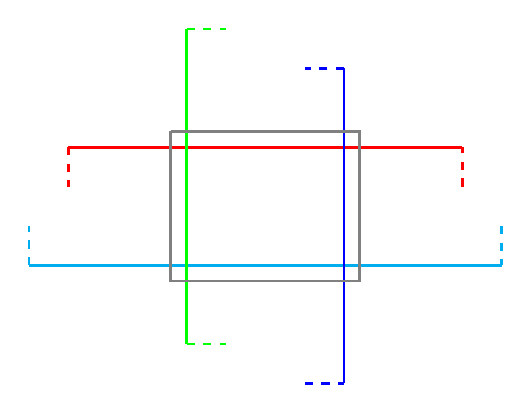
\begin{tikzpicture}[scale=1]
\draw [line width=1pt,color=red] (-2.5,1.5)-- (2.5,1.5);
\draw [line width=1pt,dash pattern=on 3pt off 3pt,color=red] (-2.5,1.5)-- (-2.5,1.0);
\draw [line width=1pt,dash pattern=on 3pt off 3pt,color=red] (2.5,1.0)-- (2.5,1.5);
\draw [line width=1pt,color=cyan] (-3,0)-- (3,0);
\draw [line width=1pt,dash pattern=on 3pt off 3pt,color=cyan] (-3,0)-- (-3,0.5);
\draw [line width=1pt,dash pattern=on 3pt off 3pt,color=cyan] (3,0.5)-- (3,0);
\draw [line width=1pt,color=green] (-1,3)-- (-1,-1);
\draw [line width=1pt,dash pattern=on 3pt off 3pt,color=green] (-1,3)-- (-0.5,3);
\draw [line width=1pt,dash pattern=on 3pt off 3pt,color=green] (-1,-1)-- (-0.5,-1);
\draw [line width=1pt,color=blue] (1,2.5)-- (1,-1.5);
\draw [line width=1pt,dash pattern=on 3pt off 3pt,color=blue] (1,2.5)-- (0.5,2.5);
\draw [line width=1pt,dash pattern=on 3pt off 3pt,color=blue] (0.5,-1.5)-- (1,-1.5);
\draw [line width=1pt,color=gray] (-1.2,1.7)-- (1.2,1.7) -- (1.2, -0.2)-- (-1.2, -0.2) -- (-1.2,1.7);
%\draw [line width=1pt,color=red] (-1.5,2)-- (-1.5,-1.2);
%\draw [line width=1pt,dash pattern=on 3pt off 3pt,color=red] (-1.5,2)-- (-1.3,2);
%\draw [line width=1pt,dash pattern=on 3pt off 3pt,color=red] (-1.3,-1.2)-- (-1.5,-1.2);
\end{tikzpicture}
\end{figure*}

考虑剩余的那个矩形$X$, 它要包含这个相交区域, 我们从 $S$ 的四个边界往外走, 如果有一个方向, 不妨假设往左走, $X$ 排在第三或更靠后, , 那么可以选择构成 $S$ 左边界的矩形与 $X$ 构成 $A_4, A_5$, 剩下三个矩形相交的部分上,下,右三个方向边界与 $S$ 一样, 左边界被推到了排第二的地方, 相比于 $S$ 多出来的那部分也被 $X$ 完全覆盖. 

反之, 如果四个方向往外走, $X$ 都是排在第二的位置, 那么我们选 $X$ 和任意两个矩形作为 $A_1, A_2, A_3$, 例如选构成 $S$上下边界的矩形. 这样三个矩形的相交区域具有上下两个方向的最"靠内"值, 左右两个方向有第二"靠内"值. 而 $A_4, A_5$ 的并集在左右两个方向至少包含了第三"靠内"的范围, 而上下两个方向也是至少包含第三靠内的范围. 所以这种情况也得证.

~ 

\noindent 严谨的证明

设每个矩形的上下左右边界对应的 $xy$ 值为 $(u_i, d_i, l_i, r_i)$. 若 $A_1 \cap A_2 = \varnothing$, 则以下 4 式至少有一个成立:
\begin{align*}
l_1 &> r_2, \\
r_1 &< l_2, \\
d_1 &> u_2, \\
u_1 &< d_2.
\end{align*}
若 $A_1\cap A_2 \neq \varnothing$, 则上述 4 式全不成立. 即有:
\begin{align*}
l_1 &< r_2, \\
l_2 &< r_1, \\
d_1 &< u_2, \\
d_2 &< u_1.
\end{align*}
为表述方便, 取等号即两边正好重合先不讨论.

同时显然存在以下关系:
\begin{align*}
l_i &< r_i, \\
d_i &< u_i.
\end{align*}
进一步可得, 若 $A_i\cap A_k\neq\varnothing,\ i,k\in\{1,2,3,4,5\}$, 则 $l_k < r_i, d_k < u_i$, 即:当任意两个矩形相交非空时, 所有矩形的"左边"在所有矩形的"右边"之左, 所有矩形的"上边"在所有矩形的"下边"之上.
可以反证, 若上述结论不成立, 譬如 $A_1$ 的"左边"在 $A_2$ 的"右边"之右, 则 $A_1$ 与 $A_2$ 的相交为空, 这与"任意两个矩形相交非空"矛盾.

若两个矩形 $A_1, A_2$ (或其他两个矩形) 相交非空, 其交集也是边平行于坐标轴的矩形, 记作 $B_{12}$, 它的"上边"为 $\min(u_1, u_2)$, "下边"为 $\max(d_1, d_2)$, "左边"为 $\max(l_1,l_2)$, "右边"为 $\min(r_1, r_2)$. 反之, 若矩形四边满足上述条件, 则该矩形必为 $A_1, A_2$ 的交集. 3个, 4个或5个矩形的交集同理.

下面分情况讨论.

1. 若存在两个矩形区域不相交 (交集为空), 譬如 $A_1\cap A_2=\varnothing$, 则 $(A_1\cap A_2\cap A_3)=\varnothing$, 而空集是任意非空集合的子集, 即 $ \varnothing\subset(A_4\cup A_5) $, 于是当存在两个不相交的矩形时, $(A_1\cap A_2\cap A_3) \subset (A_4\cup A_5)$ 成立. 


2. 若不存在两个相交为空的矩形, 即5个矩形中任意两个矩形相交都非空, 由前述结论, 记5个矩形的交集为 $B_{12345}$, 其"上边"为 $\min\{u_i\}$, "下边"为 $\max\{d_i\}$, "左边"为 $\max\{l_i\}$, "右边"为 $\min\{r_i\}$. 

2.1 若 $B_{12345}$ 的各边同属于5个矩形中的一个, 两个, 或三个, 譬如 $A_1, A_2, A_3$, 设 $B_{12345}$ 的上下左右边的$xy$值为 $u,d,l,r$, 此时显然有:
\begin{align*}
u &= \min(u_1, u_2, u_3), \\
d &= \max(d_1, d_2, d_3), \\
l &= \max(l_1, l_2, l_3), \\
r &= \min(r_1, r_2, r_3).
\end{align*}
即 $B_{12345} = (A_1\cap A_2\cap A_3)$, 而 $B_{12345}$ 是全部5个矩形的交集, 所以必为 $A_4, A_5$ 的子集. 故此时 $(A_1\cap A_2\cap A_3) \subset (A_4\cup A_5)$ 成立. 

2.2 若 $B_{12345}$ 的四边分别属于四个不同的矩形, 不妨设为 $A_1, A_2, A_3, A_4$, 如下图, 根据抽屉原理, 必有 $A_5$ 的四边不在 $B_{12345}$ 的四边之列.

2.2.1 假设 $A_5$ 的4条边正好在 $B_{12345}$ 的次外圈, 即 $A_5$ 只与 $u_1, r_2, d_3, l_4$ 相交.
\begin{figure*}[htbp]
\centering
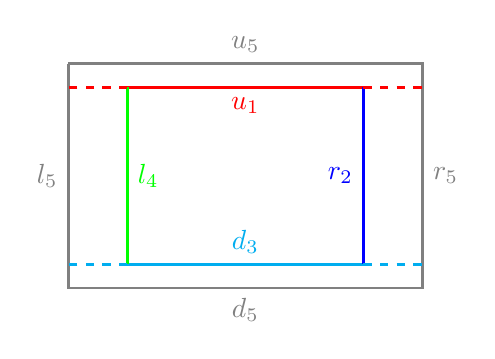
\begin{tikzpicture}[scale=1.5]
\draw [line width=1pt,color=red] (-1,1.5)-- node[below] {$u_1$} (1,1.5) ;
\draw [line width=1pt,color=cyan] (-1,0)-- node[above] {$d_3$} (1,0);
\draw [line width=1pt,color=green] (-1,1.5)-- node[right] {$l_4$} (-1,0);
\draw [line width=1pt,color=blue] (1,1.5)-- node[left] {$r_2$} (1,0);
\draw [line width=1pt,color=gray] (-1.5,1.7)--  node[above] {$u_5$} (1.5,1.7) -- node[right] {$r_5$} (1.5, -0.2) -- node[below] {$d_5$}(-1.5, -0.2) -- node[left] {$l_5$}(-1.5,1.7);
\draw [line width=1pt,dash pattern=on 3pt off 3pt,color=red] (-1,1.5)-- (-1.5,1.5);
\draw [line width=1pt,dash pattern=on 3pt off 3pt,color=cyan] (-1,0)-- (-1.5,0);
\draw [line width=1pt,dash pattern=on 3pt off 3pt,color=red] (1,1.5)-- (1.5,1.5);
\draw [line width=1pt,dash pattern=on 3pt off 3pt,color=cyan] (1,0)-- (1.5,0);
\end{tikzpicture}
\end{figure*}

显然, 
\begin{align*}
u_1 &= \min(u_1, u_3, u_5), \\
d_3 &= \max(d_1, d_3, d_5), \\
l_5 &= \max(l_1, l_3, l_5), \\
r_5 &= \min(r_1, r_3, r_5).
\end{align*}
由 $u_1, d_3, l_5, r_5$ 围成的矩形等于 $(A_1\cap A_3\cap A_5)$, 记作 $B_{135}$, 其中 $B(u_1, d_3, l_5, l_4)$ 部分, 因为 $l_5 > l_2, l_4 < r_2$, 该区域为 $A_2$ 的子集. 同理 $B(u_1, d_3, r_2, r_5)$ 部分, 因为 $r_2>l_4, r_5<r_4$, 该区域为 $A_4$ 的子集. 又因为中间部分 $B_{12345}$ 是5个矩形任意一个的子集, 所以有: $(A_1\cap A_3\cap A_5) \subset (A_2\cup A_4)$. 

2.2.2 若 $B_{12345}$ 的次外圈并不全是 $A_5$ 的四边, 譬如下图 $u_2$ 紧挨着处于 $u_1$ 之上.
\begin{figure*}[htbp]
\centering
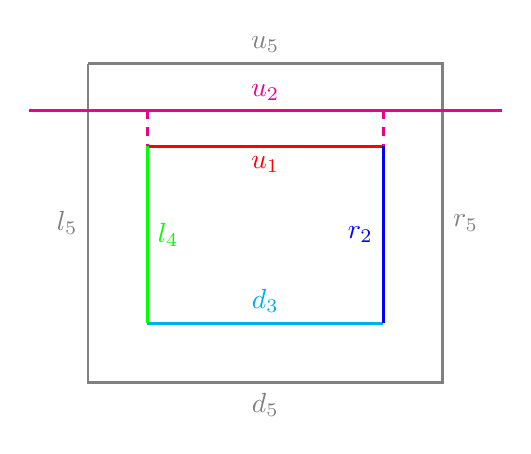
\begin{tikzpicture}[scale=1.5]
\draw [line width=1pt,color=red] (-1,1.5)-- node[below] {$u_1$} (1,1.5) ;
\draw [line width=1pt,color=cyan] (-1,0)-- node[above] {$d_3$} (1,0);
\draw [line width=1pt,color=green] (-1,1.5)-- node[right] {$l_4$} (-1,0);
\draw [line width=1pt,color=blue] (1,1.5)-- node[left] {$r_2$} (1,0);
\draw [line width=1pt,color=gray] (-1.5,2.2)--  node[above] {$u_5$} (1.5,2.2) -- node[right] {$r_5$} (1.5, -0.5) -- node[below] {$d_5$}(-1.5, -0.5) -- node[left] {$l_5$}(-1.5,2.2);
\draw [line width=1pt,color=magenta] (-2,1.8)-- node[above] {$u_2$} (2,1.8);
\draw [line width=1pt,dash pattern=on 3pt off 3pt,color=magenta] (-1,1.8)-- (-1,1.5);
\draw [line width=1pt,dash pattern=on 3pt off 3pt,color=magenta] (1,1.8)-- (1,1.5);
\end{tikzpicture}
\end{figure*}

\noindent 此时, 
\begin{align*}
u_2 &= \min(u_2, u_3, u_4), \\
d_3 &= \max(d_2, d_3, d_4), \\
l_4 &= \max(l_2, l_3, l_4), \\
r_2 &= \min(r_2, r_3, r_4).
\end{align*}
即 $B(u_2, d_3, l_4, r_2) = (A_2\cap A_3\cap A_4)$. 由图可知 $B(u_2, d_3, l_4, r_2)\subset A_5$, 即有 $(A_2\cap A_3\cap A_4) \subset (A_1\cup A_5)$.

当矩形两边重合而不重叠时, 视为相交为空集. 按照情况1处理, 或视为相交为宽度为0的特殊矩形, 按情况2处理.

综上, 原式得证.


\newpage
%------------------------------------------------------------------------------%
在城堡的周围有 9 座塔, 在夜间由若干武士把守, 每当整点的钟声响起, 每名武士均移动到下一座塔, 且移动的方向(顺时针或逆时针)始终保持不变. 已知: 

(1) 在整个夜晚, 每个武士都把守过每一座塔; 

(2) 在某一个小时中, 每座塔都被至少 2 名武士把守;

(3) 在某一个小时中, 恰有 5 座塔各有 1 名武士把守.

求证: 在某一小时中, 有一座塔无人把守.

~

解: 先证明不可能出现每座塔上同时有一个顺时针移动的武士的情况. 如果有这种情况发生, 那么每次武士移动后, 还是每座塔上都有一个顺时针移动的武士. 根据条件 (3), 落单的 5 名武士都只能是顺时针移动的, 于是所有逆时针移动的武士集中在剩余 4 座塔里, 那么这 5 名落单的武士不可能同时与逆时针移动的武士相遇, 则条件 (2) 不可能成立.

所以顺时针移动的武士至少存在一个缺口. 同理可以证明逆时针移动的武士也存在一个缺口. 以顺时针的缺口为参考点, 逆时针缺口相对顺时针缺口每次移动 2 格, 与塔数量互素. 由条件 (1) 可知每个武士至少移动了一圈, 所以缺口的位置必定有重合的时候, 缺口重合的位置即为无人把守的塔.


\newpage
%------------------------------------------------------------------------------%

\noindent 环球城市数学竞赛 1982年初中组秋季赛

一副牌 36 张按照以下顺序从上到下排列: 黑桃, 梅花, 红桃, 方块, 黑桃, 梅花, 红桃, 方块, 依此类推. 某人从上边拿起一部分牌, 上下翻转之后整体插入剩余牌堆的某个位置, 然后从牌堆顶依次4张一组的取牌. 求证: 取出的任一组4张牌都是不同花色的.

~

证明: 如果一组牌4张不同花色, 就称这组牌是协调的. 从初始牌堆任意位置取一组牌, 都是协调的. 将牌堆从上到下分为 $A,B,C$ 三部分, 每部分牌数量分别记为 $4k_1+l_1, 4k_2+l_2, 4k_3+l_3$, 其中 $k_i$ 和 $l_i$ 都是非负整数, 且 $0\le l_i \le 3$, 
\[4(k_1+k_2+k_3) + l_1+l_2+l_3 = 36 .\]

用 $A'$ 表示 $A$ 翻转之后的牌, 新牌堆从上到下依次是 $B, A', C$. 现从上往下依次取牌, 若一组牌完全在 $B$ 内, 或者完全在 $A'$ 内, 或者完全在 $C$ 内, 这组牌都是协调的. 

考虑两个交界处的牌. 第一个是 $B$ 与 $A'$ 的交界处, 这组牌记为 $X$, 若 $X$ 存在, 说明 $l_2 > 0$, $X$ 由 $B$ 最底部的 $l_2$ 张牌和 $A'$ 最顶部的 $4-l_2$ 张牌组成. 由于 $B$ 中有 $4k_2+l_2$ 张牌, 所以最底部的 $l_2$ 张牌与 $B$ 顶部的 $l_2$ 张牌花色顺序相同. 而 $A'$ 顶部的 $4-l_2$ 张牌恰好是 $A$ 底部的$4-l_2$ 张牌, 它正好跟 $B$ 顶部的 $l_2$ 张牌可以组成一组协调的牌. 所以 $X$ 是协调的. 还可能有一组位于 $A'$ 和 $C$ 的交界处, 记为 $Y$. 除 $Y$ 以外的8组牌都是协调的, 每种花色各有8张, 那么 $Y$ 中也是每个花色牌各一张, 所以也是协调的.

还有一种可能性是 $A'$ 的牌太少, 不够 $4-l_2$ 张, 说明新牌堆有一组牌横跨了 $B$ 的最底部, $A'$的全部和$C$的顶部, 将它记为 $Y$, 同样除 $Y$ 以外的所有组都是协调的, 因此$Y$ 也是协调的.


\newpage
%------------------------------------------------------------------------------%
\noindent 环球城市数学竞赛 1982年初中组秋季赛

一些物体排在一条直线上, 每个物体被染成红色或蓝色中的一种, 至少一个物体是红色, 也至少有一个是蓝色. 经过观察发现, 只要两个物体之间有10个或15个另外的物体, 那么这两个物体是同色的. 问这些物体最多有几个?

~

解: 设有$n$个物体, 编号依次为 $1,2,\cdots,n$. 不妨设 $1$ 号是红色, 当 $n=25$时, 通过广度优先遍历可以依次推出 $1, 12, 23, 17, 6, 7, 18, 22, 2, 13, 11, 24, 8, 19, 3, 14, 25, 9, 20, 4, 15$ 都是红色, 而另外4个物体 $5, 10, 16, 21$ 要同一颜色, 只要它们是蓝色就可以满足要求. 

若 $n\ge 26$, 那么由 $15$ 号物体是红色, 推出 $26$ 号也是红色, 那么 $10$ 号也要是红色, 从而 $5,10,16,21$ 都是红色, 不满足要求.

这样最大物体数量是 25.

\newpage
%------------------------------------------------------------------------------%
\noindent 环球城市数学竞赛 1983年高中组春季赛

若干个孩子围成一个圆圈, 每个孩子手中都有一些糖果. 此时, 老师给每个有奇数块糖果的孩子另外给一块糖果, 然后每个孩子都把他的一半糖果分给他左边的孩子. 不断重复以上两个步骤. 直到结果不再改变. 证明这个过程最终会终止, 从而每个孩子手中都有相同数量(偶数个)糖果.

~

证明: 第一次分糖果时, 所有孩子的糖果个数都是偶数, 设最多的有 $2M$ 个, 最少的有 $2N$ 个, 若 $M=N$, 则已经达到终止条件. 设$M>N$, 第一次分完糖果后, 每个孩子留下的糖果不会超过 $M$, 得到的糖果也不会超过 $M$, 倘若一个孩子分完糖果后手上还有 $2M$ 个糖果, 那么在下一轮老师也不会再额外给他一个糖果. 因此一次循环之后每个孩子最多还是有 $2M$ 个糖果. 

另一方面, 假设当前有 $K$ 个孩子手里有 $2N$ 个糖果, 至少存在一个手上有 $2N$ 个糖果的孩子, 传递糖果时给出了 $N$ 个糖果, 得到糖果的数目大于 $N$, 否则意味着所有孩子手上的糖果都是 $2N$. 下一轮传递糖果之前, 最多有 $K - 1$ 个孩子手里有 $2N$ 个糖果. 于是之多经过 $K$ 轮, 所有孩子手中的糖果数量都至少为 $2N+2$. 再经过若干轮, 所有孩子手中的糖果数量都至少为 $2N+4$, 等等.

以此类推, 总会在一个时刻, 所有孩子手中糖果数量都相等.

~

另一种证明方法: 设孩子人数为 $n$. 第一次分糖果时, 所有孩子的糖果个数都是偶数, 仍然设最多的有 $2M$ 个, 且由前面的思路, 一次循环过后每个孩子最多还是有 $2M$ 个糖果, 尽管老师可能会给某些孩子增加糖果, 但总会到某个时刻不再增加任何糖果(最多让$n$个孩子都有 $2M$ 个糖果).

当老师不再增加给孩子增加糖果之后, 每个孩子每次传递糖果前后手里的糖果数量都是偶数, 设传递前第 $i$ 个孩子有 $G_i$ 个糖果. 考虑$G_i$ 的平方和
\[S = G_1^2 + G_2^2 + \cdots + G_n^2 ,\]
传递前后$S$的变化为:
\begin{align*}
\Delta S &= \left(\frac{1}{2}(G_1+G_2)\right)^2 + \cdots + \left(\frac{1}{2}(G_n+G_1)\right)^2 - G_1^2 - G_2^2 - \cdots - G_n^2 \\
&= -\frac{1}{2}\left((G_1 - G_n)^2 + (G_2-G_1)^2 + \cdots + (G_n - G_{n-1})^2\right)
\end{align*}
只要不是所有的 $G_i$ 都相等, 则$\Delta S$都是严格小于 0. 而 $S$ 是非负数, 从而说明经过一定次数的传递后, 所有孩子都有相等数量的糖果.


\newpage
%------------------------------------------------------------------------------%

\noindent 1986年 IMO 第三题

给正五边形的每个顶点赋值一个整数, 使五个整数的和为正. 如果三个连续的顶点分别被赋值为 $x,y,z$, 且 $y < 0$ 那么执行下面的操作: 数字 $x,y,z$ 分别被 $x+y,-y,z+y$ 代替. 只要五个数中有一个数是负的, 就重复执行操作. 判断是否可以在有限步后结束操作.

~

解: 对于一组赋值, 定义其特征值为
\[f(x_1,x_2,x_3,x_4,x_5) = \sum_{i=1}^5{(x_{i+1}-x_{i-1})^2}. \]
其中 $x_0=x_5, x_6=x_1$.

若存在一个顶点是负数, 不妨设为 $x_3 < 0$, 则进行操作前后, 特征值的变化量为
\begin{align*}
& f(x_1,x_2+x_3,-x_3,x_4+x_3,x_5) - f(x_1,x_2,x_3,x_4,x_5) \\
= \quad & (x_2+x_3-x_5)^2 - (x_2-x_5)^2 + (x_3+x_1)^2-(x_3-x_1)^2 \\
& + (x_5+x_3)^2-(x_5-x_3)^2 + (x_4+x_3-x_1)^2-(x_4-x_1)^2 \\
= \quad & x_3(x_3+2x_2-2x_5) + 4x_3x_1 + 4x_3x_5 + x_3(x_3+2x_4-2x_1) \\
= \quad & 2x_3(x_1+x_2+x_3+x_4+x_5)
\end{align*}

因为 $x_1+x_2+x_3+x_4+x_5 > 0, x_3<0$, 所以 
\[f(x_1,x_2+x_3,-x_3,x_4+x_3,x_5) < f(x_1,x_2,x_3,x_4,x_5) .\]
又因为
\[x_1 + (x_2+x_3) + (-x_3) + (x_4+x_3) + x_5 = x_1+x_2+x_3+x_4+x_5 .\]
所以变换前后所有顶点之和不变, 都为正, 但特征值在严格变小, 而特征值是平方数之和, 最小减到 $0$, 所以一定会在有限步操作之后结束.

\newpage
%------------------------------------------------------------------------------%
\noindent Erd\H{o}s - Szekeres 定理

一个实数序列长度为 $n^2 + 1$, 并且任意两个元素都不相等. 

证明: 一定存在一个长度为 $n + 1$ 的子序列是单调递增或单调递减的.

~

这其实就是 Erd\H{o}s - Szekeres 定理. 事实上可以证明, 对于$mn + 1$个互不相同实数组成的数列 ($m,n$都是正整数), 一定存在长为 $m+1$ 的递增子列或长为 $n+1$ 的递减子列. 证明过程如下.

设序列的第 $k$ 个元素为为 $a_k$, 给每个元素赋予一组标签 $(x_k, y_k)$, 用 $x_k$ 表示以 $a_k$ 结尾的最长单调递增子序列的长度, $y_k$ 是以 $a_k$ 结尾的最长单调递减子序列的长度. 

对于任意的 $i < j$, 若 $a_i < a_j$, 则 $x_i \le x_j + 1$; 而若 $a_i > a_j$, 则 $y_i \le y_j + 1$. 因此不同元素的标签不会完全相等. 

又显然 $x_k, y_k \ge 1$, 若 $x_k \le m, y_k \le n$, 则最多只有 $mn$ 个不同标签. 于是对于长度为 $mn + 1$ 的序列, 要么存在一个 $x_k \ge m + 1$, 要么存在一个 $y_k \ge n + 1$.

~

再介绍一种构造性的证明方法. 将 $a_1, a_2, \cdots, a_{mn+1}$ 按照下面的算法放入一系列队列中:

(1) 将 $a_1$ 放入第一个队列;

(2) 对于 $a_k$, 遍历每个队列的队尾, 如果 $x_i$ 大于队尾元素, 则将 $x_k$ 放入该队列的队尾; 

(3) 若 $x_k$ 小于当前所有队列的队尾, 则新建一个队列并将 $x_k$ 放入;

(4) 回到第 (2) 步, 直到所有元素都放入某个队列.

每个队列内的元素构成一个单调递增的序列, 若所有队列都不超过 $m$ 个元素, 则队列数量至少有 $n + 1$ 个. 而对于第 $i$ 个队列($i > 1$)的任意元素来说, 总能在第 $i - 1$ 个队列中找到一个大于它的元素, 这样从最后一个队列选一个元素, 然后开始往前找, 就找到一个单调递减的序列. 于是要么存在一个长度为 $m + 1$ 的单调递增子序列, 要么存在一个长度为 $n + 1$ 的单调递减子序列.


\newpage
%------------------------------------------------------------------------------%
\noindent 2023 高考北京卷

已知 $a_1,a_2,\cdots,a_m\in\{1,2,\cdots,m\}$, 以及 $b_1,b_2,\cdots,b_m\in\{1,2,\cdots,m\}$. 

求证: 存在
$1\le p\le q\le m$ 和 $1\le s\le t\le m$, 使得: 
$$ a_p+\cdots+a_q=b_s+\cdots+b_t .$$

~

解: 当 $m=1$ 时命题显然成立. 下面考虑 $m\ge 2$ 的情况.

设数列 $\{a_i\}$ 与 $\{b_i\}$ 的前缀和分别是 $A_i$ 与 $B_i$, 即:
\begin{align*}
A_i &= a_1+a_2+\cdots+a_i \\
B_i &= b_1+b_2+\cdots+b_i 
\end{align*}

不失一般性, 可以假设 $A_m \ge B_m$. 并对每一个 $i$, 都定义一个 $i'$, 使得 
$$i'=\min\{j: A_j\ge B_i\} .$$

容易证明, 若 $1\le i < j \le m$, 有 $B_i<B_j$, 以及 $i ' \le j '$.

再定义 $M_i=A_{i'}-B_i$, 下面说明必有 $M_i < m$. 

如若不然, 即存在某个 $i$ 使得 $M_i = A_{i'}-B_i \ge m$ 的话, 那么 
$$(A_{i '} - a_{i '})-B_i \ge m - a_{i '} \ge 0 .$$

如果 $i' = 1$, 则 $A_1 - a_1 = 0$, 意味着 $B_i \le 0$, 矛盾.

如果 $i' > 1$, 则 $A_{i '} - a_{i '} = A_{i ' - 1}$,  意味着 $A_{i ' - 1} \ge B_i$, 这与 $i'$ 的取法最小性矛盾.

总之有 $0\le M_i < m$. 下面讨论 $M_i$ 可能的取值.

如果存在某个 $M_i = 0$, 也就是 $A_{i'} = B_i$, 那么只要取 $p=1$, $q=i'$, $s=1$, $t=i$, 即可得到一组满足命题条件的情况.

如果对于所有的 $M_i$, 都有 $1 \le M_i \le m-1$, 总共有 $m$ 个 $M_i$, 可能的取值只有 $m-1$ 个, 由抽屉原理必然存在两个相同的数, 假设为 $M_i = M_j$, 且 $i < j$. 得到 $A_{i '} - B_i = A_{j '} - B_j$, 亦即 $A_{j '} - A_{i '} = B_j - B_i$, 再根据前面的结论, $i '\le j '$, 并且这里不可能有 $i '=j '$, 否则 $B_j-B_i=0$ 得出矛盾. 所以只能是 $i' < j '$. 于是只要取 $p=i'$, $q=j'$, $s=i$, $t=j$, 就得到一组满足命题条件情况.

\newpage
%------------------------------------------------------------------------------%
\noindent 杂题

问题: 乒乓球队集训进行单打循环赛, 甲乙丙三人参加, 第一轮两人先打, 第三人轮空, 胜者下轮继续, 败者下场换人, 如此循环. 比赛结束后, 甲乙丙各打了15, 10, 17场, 问谁输了第二场比赛.

~

解: 三人总共打了 42 场, 所以有 21 场对局. 乙轮空了 11 场, 而一个人不会连续轮空两场. 所以只能是奇数的 11 场是乙在轮空, 意味着第二场比赛乙输了, 所以才在第三场轮空.

~

~

问题: 10 个朋友去聚餐, 围着餐桌均匀坐一圈. 所有人都坐下之后才发现桌子上有名牌, 并且每个人面前的名牌都不是自己的名字, 餐桌可以转动, 并保持各名牌的相对位置. 

证明: 可以转动餐桌, 使得同时至少有两人面前是自己的名牌.

~

解: 转动餐桌 10 下, 过程中可以让所有人都(曾经)匹配到自己的名牌, 一共发生了 10 次匹配. 但最后一次转动其实是回到初始位置, 且初始位置是没有匹配的, 所以 10 次匹配发生在前面 9 次转桌子的过程中. 由鸽笼原理可知至少有一个时刻发生了两次匹配.

~

~

问题: 平面上任意给出6个圆, 没有哪个圆覆盖别的圆的圆心.

试证: 6个圆必然没有 (同时属于所有圆的) 公共点.​​​

~

解: 任取两个圆$O_1$, $O_2$, 它们的半径分别为 $r_1$, $r_2$, 它们的公共点为 $P$. 
由于它们互不覆盖对方的圆心, 则有 $O_1O_2 > \max\{r_1, r_2\}$, 即三角形 $PO_1O_2$ 中 $O_1O_2$ 为最长边, 所以 $\angle O_1PO_2 > 60\degree$. 显然以 $P$ 为顶点作不出 6 条两两夹角超过 $60\degree$ 的射线, 故而不存在这样的公共点 $P$.

~

~

问题: 某个城市有 10 条东西向的公路和 10 条南北向的公路, 共交于 100 个路口. 小明从某个驾车路口出发, 经过每个路口恰一次, 最后回到出发点. 在经过每个路口时, 向右转不需要等待, 直行需要等待 1 分钟, 向左转需要等待 2 分钟. 问小明最少需要等待多少分钟.

~

解: 小明的路线是一条不自交的折线, 将每个路口视为一个顶点, 那么行驶路线构成一个 100 边形, 内角有可能是 $90\degree$, $180\degree$, $270\degree$, 分别对应右转, 直行, 左转. 这个多边形的内角之和为 $98\times 180\degree$, 设其中$90\degree$, $180\degree$, $270\degree$的内角个数分别是 $a,b,c$, 则
\begin{align*}
90a + 180b + 270c &= 98\times 180 \\
a + b + c &= 100
\end{align*}
可得 $a-c=4$. 等待时间为 $b+2c = 100 - a + c = 96$. 是一个固定值.

\newpage
%------------------------------------------------------------------------------%
有一堆硬币, 共 1000 枚. 将它分成两堆, 分别有 $x$ 和 $y$ 枚, 并计算乘积 $xy$. 然后对这两堆分别再分成两堆, 计算两个乘积, 例如第一堆分成$x_1+x_2$两小堆, 第二堆分成$y_1+y_2$ 两小堆, 乘积分别是 $x_1x_2, y_1y_2$. 以此类推, 直到所有堆都只有一枚硬币. 将期间得到的所有乘积加起来求和. 

求最终的和是多少? 是否与每次分堆的方式有关?

~

解: 考虑 $n$ 个变量 $a_1, a_2, \cdots, a_n$, 每个变量都赋值为 1, 被划分成$k+(n-k)$ 的两堆, 得到的乘积为:
\begin{align*}
k\cdot(n-k) &=(a_1+\cdots+a_k)(a_{k+1}+\cdots+a_n) \\
& = (a_1a_{k+1}+\cdots a_1a_n)+\cdots+(a_ka_{k+1}+\cdots+a_ka_n)
\end{align*}
展开后的项为第一堆的每一项和第二堆的每一项组合, 但两堆各自内部的变量之间没有组合. 任意一对变量$a_i, a_j$, 最初是在一堆, 并且最终要分开, 因此总会在某次划分过程中分开而得到 $a_ia_j$ 项, 并且只会得到一次.

于是最终乘积之和就是 $i\neq j$的组合个数, 为 $\dfrac{n(n-1)}{2}$. 

严格证明可以用归纳法. 归纳假设是对于一堆 $n$ 枚硬币, 通过题述方式划分得到的乘积之和为 $\dfrac{n(n-1)}{2}$, 并且与每次划分的方式无关. 证明过程略.

~

拓展问题: 有一根长度为 $L$ 的木棍, 将它分成两段, 长度分别是 $x,y$. 将两段长度相乘得到乘积 $xy$. 然后对每一段继续细分, 得到新的乘积. 重复这个过程, 直到细分到无限小, 得到的乘积也趋于无穷小. 求这个过程中所有乘积之和.

解: 在下面的直角坐标系取 $(0,L)$ 和 $(L,0)$ 两点, 构造等腰直角三角形. 斜边上取一点$(x,y)$, 满足$L=x+y$, 由这个点作到两坐标轴的垂线, 将大三角形划分成两个小等腰直角三角形和一个矩形. 矩形两边长为 $x,y$, 面积为 $xy$. 两个小三角形可以继续递归地划分下去. 随着划分过程, 剩余的三角形面积越来越小, 累加的矩形面积趋近于最初三角形的面积 $\dfrac{L^2}{2}$.
\begin{figure*}[htbp]
\centering
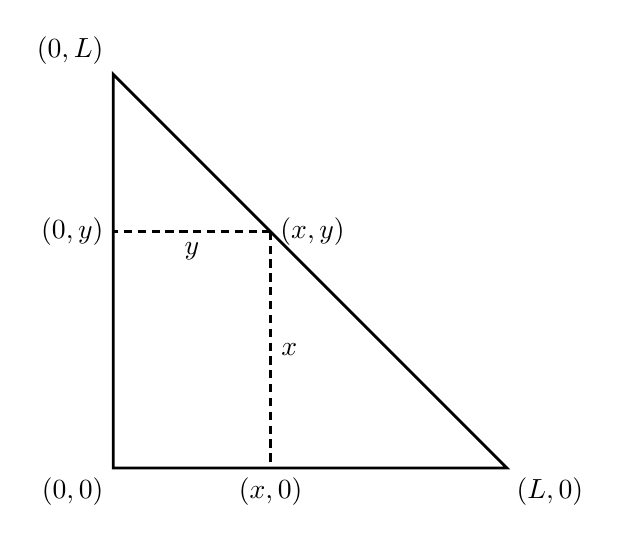
\begin{tikzpicture}[scale=1]
\coordinate[] (A) at  (0,0);
\coordinate[] (B) at (0,5);
\coordinate[] (C) at (5,0);
\coordinate[] (D) at (2,3);
\coordinate[] (E) at (2,0);
\coordinate[] (F) at (0,3);
\draw [line width=1pt] (A)--(B)--(C)-- cycle;
\draw[densely dashed,line width=1pt] (D) to [edge label = $x$](E);
\draw[densely dashed,line width=1pt] (D) to [edge label = $y$](F);
\draw[] (B) node [above left] {$(0,L)$};
\draw[] (C) node [below right] {$(L,0)$};
\draw[] (E) node [below] {$(x,0)$};
\draw[] (F) node [left] {$(0,y)$};
\draw[] (D) node [right] {$(x,y)$};
\draw[] (A) node [below left] {$(0,0)$};
%\foreach \p in {A,B,C,D}
%	\fill[fill=black,draw=black,thick] (\p) circle (1.25pt);
\end{tikzpicture}
\end{figure*}


\newpage
%------------------------------------------------------------------------------%
保险柜上有三把芯片锁, 我有这三把锁的钥匙, 但是不知道哪个钥匙对应哪个锁. 每个锁如果插入错误的钥匙, 则会锁上, 插入正确的钥匙会切换开锁和关锁的状态. 如果三把锁都打开了, 则保险柜也就自动开了, 否则无法从外界获知每个锁的状态, 初始状态也无法得知.

用怎样的策略可以保证打开保险箱?

~

解: 三把锁编号为 $1,2,3$, 三个钥匙编号为 $A, B, C$. 钥匙的所有排列分为两组: 
$$\{ABC, BCA, CAB\},$$  
$$\{ACB, CBA, BAC\}.$$ 
假设正确的排列在第一组内, 例如是 $BCA$, 在遍历对应组内的排列的过程中, 除了正确的那个排列, 同组内其他的排列三个钥匙都是全错的, 因此三个锁全部都是锁上的状态. 确保都是锁上之后继续遍历, 直到遇到正确的排列, 就会令三个锁全部打开. 这个例子中, 只要依次尝试 $ABC, BCA, CAB, ABC$, 可以找到第一组里的正确解(如果有的话). 如果正确组合在不在这组, 继续遍历第二组, 也是同样的逻辑.

一般地, 如果有 $n$ 个钥匙, 可以分出 $(n-1)!$ 个组, 依次遍历每组(第一个元素多遍历一次), 就能确保打卡所有的锁.


\newpage
%------------------------------------------------------------------------------%
漆黑的房间里有一个正方形的桌子, 它的四角各有一张牌, 可能是朝上或朝下的, 一开始不知道每张牌的状态, 我全程也无法看到任何牌. 我的目标是让这四张牌全部都变成朝上或朝下. 每一回合我可以选择任意多张牌翻转它们, 然后按一个按钮验证是不是达成目标了. 如果是, 则我胜利; 否则, 桌子会旋转一个随机的90度倍数的角度后停下, 然后开始下一回合.

我有没有策略确保胜出?

~

解: 按照下面的顺序作为每回合的操作, 8 回合内肯定能胜. 

1. 什么也不做.

2. 翻转两个对角的牌.

3. 翻转两个相邻的牌.

4. 翻转两个对角的牌.

5. 翻转一张牌.

6. 翻转两个对角的牌.

7. 翻转两个相邻的牌.

8. 翻转两个对角的牌.

然后逐一分析各种初始状态下在什么时候会获胜. 当初始所有牌都是朝上或朝下时, 第一回合就结束了. 当初始是两张上和两张下间隔排列, 则第二回合也能结束, 因为不管桌子怎么旋转, 上下间隔排列的关系不会变, 只要选对角的两张牌翻转, 所有牌的朝向就都一致了. 

如果是两张上相邻和两张下相邻, 经过第二回合, 依然还是同样的状态. 经过第三回合后, 可能直接结束, 也可能变成上下间隔排列, 这个情况到第四回合也能结束. 

因此前面四个回合可以保证初始上下各两张的时候结束. 如果上下分别有一张和三张, 经过前四个回合, 总是保持1:3或3:1 的关系. 到第五回合, 要么变成0:4, 要么变成 2:2, 要么变成 4:0. 如果是 2:2, 按前面的分析, 经过三次操作以后, 也总是能结束的.

\newpage
%------------------------------------------------------------------------------%
\noindent 来自微博

有四个棋子位于一个正方形的四个顶点上, 旋转任意两枚棋子$A,B$, 可以执行如下的"跳棋"操作: $A$ 以 $B$ 点为中心进行中心对称变换, 即 $B$ 在 $A$ 的新旧位置的中点.

问: 能够经过有限次的反复跳棋, 使四个棋子再次位于一个更大的正方形的四个顶点上?

~

解: 将平面划分成正方形网格, 使得初始时的棋子位置正好在一个单位网格的四个顶点上. 无论棋子怎么跳, 总是会落在整数格点上. 如果存在一个操作序列将小正方形变成大正方形, 将操作序列逆过来, 就可以将一个大正方形变成小正方形. 无论大正方形的朝向是正或斜, 初始的单位网格上的正方形沿用逆向操作, 将得到一个更小的正方形. 更小的正方形边长小于1, 而且它的顶点还要在整数格点上, 这是不可能的. 于是不存在将小正方形变成大正方形的操作.


\newpage
%------------------------------------------------------------------------------%

\noindent 猜多项式

Alice 和 Bob 玩一个数学游戏. Alice 秘密地写下一个多项式 $p(x)$, 多项式可以是任意次的, 但是需要满足系数是非负整数. Bob 要猜出这个多项式, 他可以问 Alice 两个问题, 他可以任选一个数 $a$, 然后 Alice 告诉他 $p(a)$ 的值, 然后他再选一个数 $b$, Alice 告诉他 $p(b)$ 的值. 

Bob 有什么策略能保证猜对?

~

解: 如果 $p(x)$ 系数比较小, 例如 $p(x) = x^2 + 2x + 1$, 那么只要 Bob 让 Alice 算 $p(10)$, 根据 $p(10) = 121$ 就可以猜到系数依次是 $1,2,1$. 这是因为将 $p(10)$ 按十进制表示出来, 每一位正好就是对应项的系数. 能这样推算的前提是每一项系数都小于 10, 否则将产生进位. 

于是, 只要 Bob 告诉 Alice 一个足够大的整数 $N$, 然后求出 $p(N)$ 值的 $N$ 进制表示, 就能得到各项系数. 只要 $N$ 大于所有项的系数, 就不会产生进位. 为了求出所有项系数的最大值, 只要知道 $p(1)$ 的值即可. 因为每一项系数都是非负整数, 所以 $N = p(1) + 1$ 一定满足大于所有系数的条件.

~

\noindent 更一般的问题:

有一个多项式各项系数都是非负实数, 给定任意实数输入, 可以得到多项式的值输出. 设计一种算法通过有限次计算得到所有系数.

\noindent 解:

假设多项式为 $p(x) = a_nx^n + a_{n-1}x^{n-1} + \cdots + a_1x + a_0$, 只要输入 $x = 0$, 就可以得到 $a_0 = p(0)$. 如果有 $p(0) = p(1)$, 可知 $p(x)$ 是常值函数. 否则, 可以定义函数 
$$g_1(x) = \frac{p(x+1) - p(1)}{x} ,$$ 
这样 $g_1(x)$ 的次数是严格小于 $p(x)$ 的次数, 并且 $g_1(x)$ 的各项系数也是非负实数. 再判断 $g_1(0)$ 是否等于 $g_1(1)$, 如果还不是, 再可以依次定义
\begin{align*}
g_2(x) &= \frac{g_1(x+1) - g_1(1)}{x} \\
g_3(x) &= \frac{g_2(x+1) - g_2(1)}{x} \\
& \cdots \\
g_n(x) &= \frac{g_{n-1}(x+1) - g_{n-1}(1)}{x} 
\end{align*}
这样每次都判断一下, 注意到 $g_k(0)$ 总是等于 $0$, 因此只要计算 $g_k(1)$ 即可. 这样总会在第 $n$ 次得到 $g_n(0) = g_n(1) = 0$, 也就是 $g_n(x)$ 是常值函数, 然后倒推, 
\[
g_{k-1}(x) = (x-1)g_k(x-1) + g_{k-1}(1) ,
\]
就可以最终得到 $p(x)$. 

例如, 假设 $p(x)=x^2+2x+1$, 因为 $p(0)=1, p(1)=4$, $p(x)$ 不是常值函数, 于是求 
\begin{align*}
g_1(1) &= p(2)-p(1) = 5, \\
g_2(1) &= g_1(2)-g_1(1) = \frac{p(3) - p(1)}{2} - g_1(1) = 1, \\
g_3(1) &= g_2(2)-g_2(1) = \frac{g_1(3) - g_1(1)}{2} - g_2(1) \\
&= \frac{p(4) - p(1)}{6} - \frac{g_1(1)}{2} - g_2(1) = 0
\end{align*}
这样就可以推断 
\begin{align*}
g_3(x) &= 0\\ 
g_2(x) &= g_2(1) = 1 \\
g_1(x) &= (x-1)g_2(x-1) + g_1(1) = x + 4\\
p(x) &= (x-1)g_1(x-1) + p(1) = x^2 + 2x + 1
\end{align*}


\newpage
%------------------------------------------------------------------------------%
Alice 和 Bob 进行一个游戏, Alice 在纸上写一个 1 到 100 之间的一个整数 $k$, 让 Bob 来猜, 若猜对了 Alice 就要支付 $k$ 元给 Bob. 问 Bob 的最佳策略是什么.

~

分析: 若 Bob 以均等的概率在 1 到 100 之间猜, 那么 Alice 应该写尽量小的数, 以最小化损失. Bob 考虑到这一点, 也会尽量猜小的数. 

假设 Alice 的策略是写下每个数的概率是 $q_1, \cdots, q_{100}$; Bob 的策略是猜每个数的概率为 $p_1, \cdots, p_{100}$. 于是他们的期望损失(或收益)为:
\[ E = \sum_{k=1}^{100}k\cdot p_k\cdot q_k ,\]

若 Alice 提前知道了 Bob 的策略 $\{p_i\}$, 他需要最小化 $E$, 为此他需要将更多的概率分配给使得 $k\cdot p_k$ 最小的那个 $k$, 例如令 $j = \mathop{\arg\min}\limits_{k}\{k\cdot p_k\}$, Alice 的策略就是令猜 $j$ 的概率 $p_j = 1$, 而猜其他数的概率都是 $p_i = 0, (i\neq j)$. 此时损失为 $E = \min\limits_{k}\{k\cdot p_k\}$. 当然如果同时有多个 $j$ 满足条件, Alice 可以在它们之间任意分配概率, 损失仍然不变.

另一方面, 从 Bob 的角度来看, 他需要最大化 $E$, 并且也已经知道 Alice 会采取上述策略, 于是 Bob 的目标是确定 $\{p_i\}$, 使得 $\min\limits_{k}\{k\cdot p_k\}$ 最大, 亦即求
\[ \max\limits_{\{p_i\}}\left( \min\limits_{k}\{k\cdot p_k\} \right),\ s.t.\ p_i\ge 0, \sum_i p_i = 1 .\]
Bob 的最佳策略应该是使得所有的 $k\cdot p_k$ 都等于同一个值, 并记这个值为 $p$, 它是 Bob 在此策略下的收益. 如 Bob 不采用这个策略, 假设对于某个 $m$, 有 $m\cdot p_m > p$, 那么必然存在一个 $n$ 使得 $n\cdot p_n < p$, 这样 Alice 就会选择猜 $n$, 而 Bob 的最大收益就是 $n\cdot p_n$, 它是小于 $p$ 的.

下面求 $p$ 和 $p_k$ 的值. 因为 $p_k = \dfrac{p}{k}$, 对于 $k=1,\cdots,100$ 成立, 而 $\sum p_k = 1$, 故
\[p = \left(1 + \frac{1}{2} + \frac{1}{3} + \cdots + \frac{1}{100}\right)^{-1} .\]
在此策略下, 期望收益为
\[ E = \sum_k(k\cdot p_k)q_k = p\sum_kq_k = p .\]

以上分析表明, Bob 知道如果存在某个对自己最有利的策略, Alice 也一定能推测出来, 并做出应对, 在此前提下, Bob 按照上述策略, 保证无论 Alice 如何应对, 自己总能获得最大的期望收益. 

对称地分析 Alice 的策略, 他写下每个数的概率也应该是 $q_k = \dfrac{p}{k}$.

总的来说, 两人都会比较倾向于写和猜较小的数, 也是符合直觉的.


\newpage
%------------------------------------------------------------------------------%
三个人 A,B,C 玩一个游戏, 每个人写下一个正整数, 谁的数字是不重复的数字里最小的就胜出, 他们用怎样的策略能让各自胜出的可能性尽可能大?

~

分析: 如果三人在 1 和 2 两个数中等概率地随机选择, 每个人获胜当且仅当另外两人选择的是与自己不同的数, 因此都是 $\dfrac{1}{4}$, 还有 $\dfrac{1}{4}$ 概率是三人选择的数相等, 从而没人胜出. 虽然每个人是对称的, 他们获胜的概率都相等, 但是可以通过减小平局发生的概率来增加每个人获胜的概率.

假设策略是每个人以概率 $p_k$ 写下数字 $k$, 例如 A 写下的是 $k$, 那么 A 获胜意味着 B和C 写下了小于 $k$ 的两个相等的数, 或者 B和C 都写下了大于 $k$ 的数(这个情况下不一定相等), 对应的概率为
\[P_k = p_1^2+p_2^2+\cdots+p_{k-1}^2+(p_{k+1}+\cdots)^2 .\]
记 $\displaystyle A_k = \sum_{i=k+1}^\infty p_i$, 有 $p_k = A_{k-1} - A_k$, 以及
\begin{align*}
P_k &= p_1^2+p_2^2+\cdots+p_{k-1}^2+A_k^2 \\
P_{k+1} &= p_1^2+p_2^2+\cdots+p_{k-1}^2+p_k^2 + A_{k+1}^2
\end{align*}
作为最优策略应该保证 A 不管写哪个数获胜的概率都相等, 如若不然, 所有人都只会选择写胜率最大的那个数, 这将导致三个人写的数相等, 从而获胜概率都是0, 不合理. 于是根据 $P_k = P_{k+1}$ 可得
\[ A_k^2 = (A_{k-1}-A_k)^2 + A_{k+1}^2 ,\]
整理得到: 
\[A_{k-1}^2 - 2A_{k-1}A_k + A_{k+1}^2 = 0.\]
初值为$A_0 = 1$. 可以设 $A_k = \lambda^k$, 得 $\lambda^4-2\lambda + 1 = 0$, 舍去一个根 $\lambda = 1$, 有
\[ \lambda^3 + \lambda^2 + \lambda - 1 = 0 .\]
令 $f(\lambda) = \lambda^3 + \lambda^2 + \lambda - 1$, 则 $f'(\lambda) = 3\lambda^2 + 2\lambda + 1$ 在 $\lambda \in (0,1)$ 上恒为正, 说明 $f(\lambda)$ 单调递增, 而 $f(\dfrac{1}{2}) < 0, f(1) > 0$, 说明 $\lambda > \dfrac{1}{2}$. 事实上可以由三次方程求根公式算出 $\lambda$ 的值.

得到$\lambda$, 可计算策略为 $p_k = A_{k-1}-A_k = \lambda^{k-1}(1-\lambda)$, 并且每个人获胜的概率为
\[P_1 = A_1^2 = \lambda^2 > \frac{1}{4} .\]
可见这个策略确实对每个人的胜率都是有提升的.


\newpage
%------------------------------------------------------------------------------%
\noindent 纳什均衡

Alice 和 Bob 玩一个猜拳游戏, 每个人可以选择出 1 点或 4 点, 如果两人数字之和是奇数则 Alice 胜, 是偶数则 Bob 胜. 胜者可以获得两人所出数字之和的分数. 问这个游戏是否公平, 以及两人的策略是什么.

~

解: 假设 Alice 和 Bob 分别以概率 $p$ 和 $q$ 出 1, 以 $1-p$ 和 $1-q$ 的概率出 4. 则每一局两人的期望得分分别是 
\begin{align*}
S_A &= p(1-q)\cdot 5 + q(1-p) \cdot 5 = 5p+5q-10pq \\
S_B &= pq \cdot 2 + (1-p)(1-q)\cdot 8 = 8-8p-8q+10pq
\end{align*}

每个人的目标是让自己的得分比对方的得分多, 对于 Alice, 他希望最大化 $S_A - S_B$ 的值, 即
\[D = S_A - S_B = 13p + 13q - 20pq - 8 = 13p - 8 + (13-20p)q ,\]

而 Bob 的目标则是最小化上面的值. 如果上式 $q$ 的系数不为 0, Bob 都可以通过选择 $q$ 的来让 $D$ 最小, 又因为 $D$ 关于 $q$ 是线性的, 所以 Bob 的策略是根据 $13 - 20p$ 的正负号选择 $q$ 是 0 或 1, 相当于是一个固定策略. 但一旦 Bob 的策略固定, Alice 也能采取相应的固定策略应对. 例如, 若 Alice 推测 Bob 固定选 1, Alice 的最佳策略是固定选 4, Bob 也能推测出这一点, 也要改成固定选 4, 此时 Alice 又要改成固定选 1. 不能达到平衡.

所以只能是 $13 - 20p = 0$, 这样无论 Bob 采用什么策略, $D$ 的值是固定的, 反过来也一样, 这就达到了纳什均衡状态: 任何人单方面修改策略都不能让自己的收益更大(在本例中也是让对方收益更小). 纳什均衡下, Alice 的策略是以 $\dfrac{13}{20}$ 概率出 1, 以 $\dfrac{7}{20}$ 出 4. 这样单局比 Bob 期望能多得 0.45 分. 

从这里也可以看出这个游戏不是公平的, 对 Alice 更有利.

\newpage
%------------------------------------------------------------------------------%
\noindent 囚犯猜数问题系列

\noindent 问题:

Alice 和 Bob 被抓进监狱, 邪恶的典狱长邀请他们玩一个游戏, 下面是游戏规则: 两人将被关进不同的牢房, 每天他们两人要分别抛一次硬币, 并猜对方的硬币朝向, 如果两人都猜错, 就要接受惩罚. Alice 和 Bob 在关进牢房前有一次机会商量对策, 之后不允许有任何交流. 他们是否有策略能避免惩罚.

~

\noindent 解: 

只要 Alice 猜的是自己硬币的朝向, Bob 猜的是自己硬币的反向即可. 若两人硬币朝向一样, 则 Alice 正确. 若两人硬币朝向相反, 则 Bob 正确. 这样两人中总有一人猜对.

~

\noindent 问题:

邪恶的典狱长随便找了一个罪名, 将 16 个囚犯带到了审讯室, 说: 

``你们要为自己的罪行付出代价, 不过, 出于仁慈, 我再给你们一个机会. 我会给你们每个人背后贴一张纸, 纸上的数字从 1 到 16 都有可能, 不同人的数字可能重复. 你们每个人都可以转过身给别人看自己背上的数字, 但期间你们不许无故发出任何声音, 做任何其他动作. 之后警卫会依次把你们带到我的办公室, 告诉我你自己背后的数字是多少. 只要你们 16 人中有一人猜对自己背后的数字, 我就既往不咎, 但如果你们都猜错了, 就要接受严厉的惩罚. 我最后再给你们 5 分钟商量对策. 5 分钟后就不许再发出声音. 同时, 如果游戏过程中有任何人做出令人生疑的好似传递信息和暗示的举动, 所有人也要接受惩罚.''

他们该用怎样的策略来避免惩罚呢?

~

\noindent 解: 

为讨论方便起见, 将每个人编号为 $0,1,2,\cdots,15$, 后面的计算中, 每个人看到的其他人背后的数字也减去 1, 这样背后数字的范围也是 0 到 15. 

设第 $i$ 个人背后数字为 $a_i$, $i$ 和 $a_i$ 都可以用 4 位二进制数表示. 用 $\oplus$ 表示按位异或运算, 并假设所有人背后数字按位异或起来结果是 $s$, 即:
\[s = a_0 \oplus a_1\oplus \cdots \oplus a_{15} .\] 
虽然第 $i$ 个人看不到自己背后的数字, 也无法计算出 $s$, 但是可以通过看其他人背后的数字算出 $s\oplus a_i$ 的值, 因为按位异或运算满足交换律和结合律, 且任何数与自己按位异或都得到 0, 所以
\begin{align*}
s\oplus a_i &= a_0\oplus\cdots a_{i-1}\oplus (a_i\oplus a_i) \oplus a_{i+1}\oplus\cdots\oplus a_{15}\\
&= a_0\oplus\cdots a_{i-1}\oplus a_{i+1}\oplus\cdots\oplus a_{15}
\end{align*}
也就是只要将其他人背后的数字累积使用按位异或运算, 就可以得到 $s\oplus a_i$. 

进而, 只要每个人都计算并回答 $(s\oplus a_i) \oplus i$, 因为编号已经覆盖了 $s$ 的取值范围, 不管 $s$ 是多少, 它总会等于某个人的编号 $j$. 那么对于第 $j$ 个人来说, $s\oplus j = 0$, 所以
\[s\oplus a_j \oplus j = s\oplus j \oplus a_j = a_j .\]
于是总有一个人能答对.

~

\noindent 推广: 

如果囚犯人数和背后的数字范围不是2的幂次, 该如何应对?

思路还是类似, 假设人数为 $n$, 每个人背后数字是 $[0,n-1]$ 范围内的一个整数. 考虑整数的模 $n$ 加法群 $\mathbb{Z}_n$, 下面的加减法都是在模 $n$ 意义下讨论. 记所有人背后数字之和是 $s$, 即
\[s \equiv \sum_{i=0}^{n-1}a_i \pmod{n} .\] 
每个人仍然将他看到的其他人背后数字求和, 第 $i$ 个人的计算结果是 $r_i = s-a_i$, 只要他回答 $g_i = i-s_i$, 那么总是存在一个 $j=s\in[0,n-1]$, 满足:
\[g_j = j - r_j = j - (s - a_j) = a_j .\]
所以第 $j$ 个人回答的结果正好等于其背后的数字.


\newpage
%------------------------------------------------------------------------------%
两人各自在 $1,2,\cdots,N$ 内选一个数, 秘密地写在纸上, 然后一起亮出来比较. 如果两数相差1, 则较小者获胜, 如果相等则是平局, 其他情况都是较大者获胜. 

问最好的策略是什么.

~

解: 若 $N=3$, 则跟石头剪刀布等价, 对应决策收益矩阵的如下, 其中行表示 $A$ 的决策, 列表示 $B$ 的决策, 矩阵内容表示 $A$ 的收益.
\begin{figure*}[htbp]
\centering
\setlength\extrarowheight{3pt}
\begin{tabular}{|c|c|c|c|}
\hline
\diagbox[]{A}{B}  & 1(石头)    & 2(剪刀)    & 3(布)    \\ \hline
1(石头) & 平    & 胜 & 负 \\ \hline
2(剪刀) & 负 & 平    & 胜   \\ \hline
3(布)  & 胜  & 负 & 平    \\ \hline
\end{tabular}
\end{figure*}

考虑 $N = 4$ 的情况,  从下表可以看出, 不管 $B$ 怎么选, 对于 $A$ 而言, 选 4 的结果都不比选 1 差, 所以 $A$ 不会选 1. 同理对 $B$ 也是这样.
\begin{figure*}[htbp]
\centering
\setlength\extrarowheight{3pt}
\begin{tabular}{|c|c|c|c|c|}
\hline
\diagbox[]{A}{B}  & 1    & 2   & 3 & 4    \\ \hline
1 & 平    & 胜 & 负 & 负 \\ \hline
4  & 胜  & 胜 & 负 & 平    \\ \hline
\end{tabular}
\end{figure*}

于是这又回到了在三个数之间选择的问题. 

对于 $N=5$ 的情况也是一样, 选 5 总是不比选 1 和 2 差, 最后实际上也是只能在三个数之间选. 

所以最好的策略就是在 $N-2, N-1, N$ 三个数之间随机选.


\newpage
%------------------------------------------------------------------------------%
$A,B$ 两队比赛, 最多 7 场, 谁先胜 4 场则停止比赛. 每场比赛都可以单独押注任意金额, 押对了当场的结果则从庄家处赢得等量的钱, 否则输掉赌注. 某人最初手里有 100 元, 他是 $A$ 队的支持者, 每场比赛只押 $A$ 队胜, 想要在所有比赛结束时, 若 $A$ 队获得最终冠军, 则赢得 100 元, 否则输掉 100 元. 

例如可以在第一场就将 100 全押出去, 如果输了则全部损失, 即使后面 $A$ 又赢了 4 场, 获得最终冠军, 但他没有赢得 100 元, 因此不符合要求.

那么要怎样安排每场比赛的押注? 注意比赛可能进行 4,5,6,7 场. 

~

解: 用 $(x,y)$ 表示两队的比分, 从后往前分析. 在 $(3,3)$ 时, 若下一场 $A$ 胜要赢 100 元, $B$ 胜要输 100 元, 所以此人手里应该要有 100 元, 并全部押上. 到达 $(3,3)$ 之前, 可能是 $(2,3)$ 或者 $(3,2)$. 考虑 $(2,3)$, 需要在到达 $(3,3)$ 时手里有 100 元, 到达 $(2,4)$ 时手里有 0 元. 因此 $(2,3)$ 时手上应该有 50元, 并押注 50 元. 而在 $(3,2)$ 时, 需要在到达 $(3,3)$ 时有 100元, 到达 $(4,2)$ 时有 200 元. 因此 $(3,2)$ 时手上应该有 150 元, 押注 50元.

下表内第一行和第一列表示两队分别的得分, 内部值是各个比分下此人手中应有的钱. 先填上边界情况. 
\begin{figure*}[htbp]
\centering
\setlength\extrarowheight{3pt}
\begin{tabular}{|c|c|c|c|c|c|}
\hline
\diagbox[]{A}{B}  & 4    & 3   & 2 & 1 & 0    \\ \hline
4 &  -  & 200 & 200 & 200 & 200 \\ \hline
3  & 0  &   &   &  &    \\ \hline
2  & 0  &   &   &  &    \\ \hline
1  & 0  &   &   &  &    \\ \hline
0  & 0  &   &   &  &    \\ \hline
\end{tabular}
\end{figure*}

若某个格子左边和上边的值都确定了,那么这个格子的值也确定了. 从 $(3,3)$ 开始填表, 最终如下:
\begin{figure*}[htbp]
\centering
\setlength\extrarowheight{3pt}
\begin{tabular}{|c|c|c|c|c|c|}
\hline
\diagbox[]{A}{B}  & 4    & 3   & 2 & 1 & 0    \\ \hline
4 &  -  & 200 & 200 & 200 & 200 \\ \hline
3  & 0  & 100 & 150 & 175 & 187.5 \\ \hline
2  & 0  & 50 & 100 & 137.5 & 162.5 \\ \hline
1  & 0  & 25 &  62.5 & 100 & 131.25  \\ \hline
0  & 0  & 12.5 & 37.5 & 68.75 &  100  \\ \hline
\end{tabular}
\end{figure*}
从每个格子往左走表示 $B$ 胜, 往上走表示 $A$ 胜, 因此这三个格子需要构成一个等差数列, 公差就是在对应状态下的赌注.


\newpage
%------------------------------------------------------------------------------%
数轴上有一些点, 都往正方向匀速运动. 若两个点相遇了, 会合并成一个点, 并以原先较慢的那个点的速度继续前进. 若开始有 $n$ 个点在数轴上的不同位置, 两两之间速度不相同. 最终期望会变成多少个点. 期望指的是对一切初始排列的可能性取平均.

解: $n$ 个点初始有 $n!$ 种排列, 将所有排列最终剩余的点个数相加得到 $s_n$, 那么期望就是 
\[a_n = \frac{s_n}{n!}.\]

对于 $n = 1$, $s_n = 1$, $a_1 = 1$.

对于 $n = 2$, 若是 $1,2$ 排列, 剩余 $2$ 个点, 若是 $2,1$ 排列, 剩余 $1$ 个点, $s_2 = 3$, $a_2 = \dfrac{3}{2}$.

对于 $n = 3$, 有如下情况:
\begin{figure*}[htbp]
\centering
\setlength\extrarowheight{3pt}
\begin{tabular}{|c|c|}
\hline
排列 & 剩余 \\ \hline
1,2,3 & 3 \\ \hline
1,3,2 & 2 \\ \hline
2,1,3 & 2 \\ \hline
2,3,1 & 2 \\ \hline
3,1,2 & 1\\ \hline
3,2,1 & 1 \\ \hline
\end{tabular}
\end{figure*}
从而 $s_3 = 11, a_3 = \dfrac{11}{6} = 1 + \dfrac{1}{2} + \dfrac{1}{3}$.

于是猜测 $$a_n = 1 + \dfrac{1}{2} + \cdots + \dfrac{1}{n}.$$ 
下面用归纳法证明. 

前面分析对 $n=1,2,3$ 都成立. 假设对 $n = k (\ge 3)$ 成立, 对于 $n = k+1$, 将最快的那个点单独考虑, 余下 $k$ 个点. 若最快的点在最前面, 则不会被剩下的点追上, 这样的情况数共有 $k!$ 种, 剩余点数总数为 $(a_k+1)k!$. 

若最快的点不在最前面, 共有 $k\cdot k!$ 种可能, 不管它在哪个位置, 都会追上前面那个点, 并变回只有 $k$ 个点的情况. 此时剩余点数总数为 $k\cdot k!\cdot a_k$. 

两部分加起来, 得
\[a_{k+1} = \frac{s_{k+1}}{(k+1)!} = \frac{(a_k+1)k! + k\cdot k!\cdot a_k}{(k+1)!} = a_k + \frac{1}{k+1} .\]
说明归纳假设对 $n = k+1$ 也成立.




















